\section{Introduction}
\label{sec:introduction}

Laplacian Eigenmaps (LE)~\citep{belkin03a} is a method for nonlinear dimensionality reduction and data representation. Given data points $\{X_1,\ldots,X_n\} \subset \Reals^d$, LE maps each $X_i$ to a vector $(v_{1,i},\ldots,v_{K,i})$ according to the following steps.
\begin{enumerate}
	\item First, LE forms a \emph{neighborhood graph} $G = (V,W)$ over the points $\{X_1,\ldots,X_n\}$. The graph $G$ is an undirected, weighted graph, with vertices $V = \{X_1,\ldots,X_n\}$, and weighted edges $W_{ij}$ which correspond to the proximity between points $X_i$ and $X_j$.
	\item Next, LE forms an (unweighted) \emph{graph Laplacian} matrix $L \in \Reals^{n \times n}$, a symmetric and diagonally dominant matrix with diagonal elements $L_{ii} = \sum_{j = 1}^{n} W_{ij}$, and off-diagonal elements $L_{ij} = -W_{ij}$. 
	\item Finally, LE takes the eigendecomposition $L = \sum_{k = 1}^{n} \lambda_k v_k v_k^{\top}$, and outputs the vectors $(v_{1,i},\ldots,v_{K,i}) \in \Reals^K$ for each $i = 1,\ldots,n$.
\end{enumerate} 
A natural way to use LE is by taking the vectors $\{(v_{1,i},\ldots,v_{K,i})\}_{i = 1}^{n}$ to be features in a downstream regression algorithm. In this paper, we study a simple method along these lines: Principal Components Regression with Laplacian-Eigenmaps (PCR-LE), a method for nonparametric regression which operates by running ordinary least squares (OLS) using the features output by LE. Given pairs of design points and responses $(X_1,Y_1),\ldots, (X_n,Y_n)$, PCR-LE computes an estimate $\wh{f} \in \Reals^n$,
\begin{equation}
\label{eqn:pcr-le}
\wh{f} := \argmin_{f \in \mathrm{span}\{v_1,\ldots,v_K\}} \|{\bf Y} - f\|_2^2
\end{equation}
where ${\bf Y} = (Y_1,\ldots,Y_n) \in \Reals^n$ is the vector of responses and $\|\cdot\|_2$ denotes the usual Euclidean norm in $\Reals^n$. (For a formal definition of LE and PCR-LE, see Section~\ref{subsec:laplacian_eigenmaps}.)

LE has been practically very successful, and by now has been used for various statistical tasks such as spectral clustering, manifold learning, level-set estimation, semi-supervised learning, etc. At this point there exists a rich literature \citep{koltchinskii2000,belkin07,vonluxburg2008,burago2014,shi2015,singer2017,garciatrillos18,trillos2019, calder2019, cheng2021,dunson2021} explaining this practical success from a theoretical perspective. Loosely speaking, these works model the design points as being independent samples from a distribution $P$ with density $p$, and show that in this case the eigenvectors of the graph Laplacian $L$ are good empirical approximations of population-level objects. These population-level objects are eigenfunctions $\psi_k$---meaning solutions, along with eigenvalues $\rho_k$, to the equation $\Delta_P \psi_k = \rho_k \psi_k$--- of a density-weighted Laplacian operator defined via:
\begin{equation}
\label{eqn:density-weighted-laplace}
\Delta_Pf := -\frac{1}{p}~ \mathrm{div}(p^2 \nabla f).
\end{equation}  
(Here $\mathrm{div}$ stands for the divergence operator, and $\nabla$ for the gradient. See~\eqref{eqn:laplace_beltrami_eigenproblem} for the formal definition of eigenpairs $(\rho_k,\psi_k)$.) These eigenfunctions in turn characterize various interesting structural aspects of $p$, such as the location and number of high- and low-density regions, the shape and intrinsic dimension of its support, and so forth.

These aforementioned works justify LE as method for data representation, by establishing that each feature vector $(v_{1,i},\ldots,v_{K,i})$ serves an empirical approximation to an idealized representation $(\psi_1(X_i),\ldots,\psi_K(X_i))$. They also provide quantitative guarantees for the accuracy with which LE approximates this ideal representation. However, this theory does not focus on the statistical properties of PCR-LE for classical regression problems such as estimation and testing. That is the major question we address in this paper. We adopt the usual model of nonparametric regression with random design, where one observes independent pairs $(X_1,Y_1),\ldots,(X_n,Y_n)$ of design points and responses. We assume the design points $\{X_1,\ldots,X_n\}$ are sampled from an unknown distribution $P$ supported on $\mc{X} \subseteq \Rd$, and the responses follow a signal plus Gaussian noise model,
\begin{equation}
\label{eqn:model}
Y_i = f_0(X_i) + w_i, \quad w_i \sim N(0,1),
\end{equation}
with noise variables $w_i$  independent of design points $X_i$. The task is to learn the regression function $f_0$, which is unknown but assumed to belong to a Sobolev space $H^s(\mc{X})$. We consider two settings: one where $\mc{X}$ is a full-dimensional domain, and the other where $\mc{X}$ is a low-dimensional submanifold of $\Rd$. In each setting, we derive upper bounds which imply that the PCR-LE estimate $\wh{f}$, and a test using the statistic $T = \|\wh{f}\|_2^2$, are statistically optimal methods for two classical problems in nonparametric regression: estimation and goodness-of-fit testing.  

% (AG 10/28/21): I comment out the paragraph below. I decided the better approach was to first give our results, then comment on their perspective. 
% At first glance, the optimality of PCR-LE is surprising. As a function of the sample size $n$, known rates of convergence of LE are much slower than the minimax optimal rates of convergence over $H^s(\mc{X})$ (roughly speaking $n^{-2s/(2s + d)}$ for estimation and $n^{-4s/(4s + d)}$ for testing). This is not due to suboptimal theory for LE. Rather, it reflects a fundamental fact: \emph{for this problem, regression using learned features does not rely on accurately learning the features}. It is essential to employ modes of analysis which exploit this fact in order to derive sharp rates of convergence for PCR-LE. We explain this in more detail after summarizing our main results.

\paragraph{Sobolev spaces and spectral series regression.}
To analyze PCR-LE, we work in a classical situation where the regression function is assumed to belong to a (Hilbert-)Sobolev space. For an open domain $\mc{X} \subseteq \Rd$, the Sobolev space $H^s(\mc{X})$ consists of all functions $f \in L^2(\mc{X})$ which are $s$-times weakly differentiable, with all order-$s$ partial derivatives $D^{\alpha}f \in L^2(\mc{X})$. We study regression over Sobolev spaces in part because, generally speaking, the minimax rates are well-understood; as mentioned before, when the domain $\mc{X}$ is full-dimensional they are $n^{-2s/(2s + d)}$ for estimation, and $n^{-4s/(4s + d)}$ for testing. For this reason, regression over Sobolev spaces is a good setting in which to see whether PCR-LE measures up to more standard minimax optimal approaches, which have strong theoretical guarantees but are less often used in practice. We give a more specific comparison between PCR-LE and some of these more classical methods in Section~\ref{sec:discussion}.

We also view PCR-LE as being particularly well-suited for regression over Sobolev spaces due to their close connection with \emph{spectral series regression}. Spectral series regression computes generalized empirical Fourier coefficients $\wt{a}_k := \frac{1}{n}\sum_{i = 1}^{n} Y_i \psi_k(X_i)$, and truncates to the $K$-lowest frequency eigenfunctions of $\Delta_P$, producing the estimate
\begin{equation}
\label{eqn:population-level_spectral_series}
\wt{f}(x) = \sum_{k = 1}^{K} \wt{a}_k \psi_k(x).
\end{equation} 
Spectral series regression is intrinsically linked with Sobolev spaces. That is because under appropriate boundary conditions, a unit ball in the order-$s$ Sobolev space consists of functions $f = \sum_{k} a_k \psi_k \in L^2(\mc{X})$ for which the generalized Fourier coefficients $\{a_k\}_{k = 1}^{\infty}$ satisfy the decay condition $\sum_{k} a_k^2 \rho_k^s \leq C$ (See Section~\ref{subsec:spectral_projection} for more details). This decay condition justifies the truncated series estimator \eqref{eqn:population-level_spectral_series}, since it means the truncation will incur only a limited amount of bias for any $f_0 \in H^s(\mc{X})$. For this reason spectral series regression over Sobolev spaces has been well-studied---at least when $\mc{X} = [0,1]^d$---since at least \citet{rice1984},\footnote{And proposed much earlier in the context of density estimation by \citet{cencov1962}.} and its optimality properties are by this point generally well-understood.

PCR-LE serves as an empirical approximation to spectral series regression, since as already mentioned the eigenvectors $v_k$ are empirical approximations to the eigenfunctions $\psi_k$ of $\Delta_P$. Viewed in this light, a major advantage of PCR-LE is that it operates without needing knowledge of the design distribution $P$. This is an advantage because in our context $P$ is treated as an unknown and potentially complex distribution, and for example can be highly non-uniform, have a complicated support which may be a submanifold of $\Rd$, or both. In contrast, spectral series regression relies on diagonalizing the density-weighted Laplacian $\Delta_P$, and in our context must be viewed as an oracle method; to emphasize this we henceforth refer to the estimator defined in~\eqref{eqn:population-level_spectral_series} as \emph{population-level spectral series regression}. On the other hand, intuitively PCR-LE incurs some extra error by using an empirical approximation to the underlying basis $\{\psi_k\}_{k = 1}^{\infty}$: our work shows that in many cases, this extra error is not enough to change the overall rate of convergence.

\subsection{Main contributions}
Summarized succinctly, our main contribution is to theoretically analyze nonparametric regression with PCR-LE and establish upper bounds which imply that this method often achieves optimal rates of convergence over Sobolev spaces.

\paragraph{Rates of convergence: population-level spectral series regression.}
As we have already mentioned, the minimax optimal rates over Sobolev spaces are generally well-known, as are upper bounds for population-level spectral series methods which match these rates. However, we could not find precisely stated results applying to our setting, which is quite general in the following respects.
\begin{enumerate}
	\item We consider Sobolev spaces $H^s(\mc{X})$ for all combinations of $s$ and $d$. This includes the subcritical regime where the smoothness parameter $s$ satisfies $s < d/2$; in this regime $H^s(\mc{X})$ does not continuously embed into the space of continuous functions $C^0(\mc{X})$.
	\item We consider general design distributions $P$, which may satisfy certain regularity conditions but are not limited to being, say, the uniform distribution over $[0,1]^d$. 
\end{enumerate}
For completeness, we analyze population-level spectral series methods in this general setting, and establish upper bounds showing that such methods converge at the ``usual'' rates of $n^{-2s/(2s + d)}$ for estimation and $n^{-4s/(4s + d)}$ for testing. This analysis relies heavily on certain asymptotic properties of the continuum eigenfunctions $\psi_k$ and eigenvalues $\rho_k$, which hold for quite general second-order differential operators $\mc{L}$ including the density-weighted Laplacian $\mc{L} = \Delta_P$.

\paragraph{Rates of convergence: PCR-LE.}
The rest of our results consist of various upper bounds on the rates of convergence for the PCR-LE estimator $\wh{f}$, and a test using the statistic $\wh{T} = \|\wh{f}\|_2^2$. These upper bounds quantify two important properties of PCR-LE: first, that it can take advantage of smooth higher-order derivatives, and second that it can adapt to low intrinsic dimension of the design distribution, each in an optimal manner. We consider two models for the design distribution $P$, the flat Euclidean and manifold models (See Section~\ref{subsec:regression_laplacian_eigenmaps} for the formal definitions of these models). In the first model, the design distribution $P$ has support $\mc{X}$ which is a full-dimensional set in $\Rd$. In this case, our main contributions are as follows:
\begin{itemize}
	\item  Over a ball in the Sobolev space $H^{s}(\mc{X})$, we establish that the PCR-LE estimator $\wh{f}$ has in-sample mean-squared error on the order of $n^{-2s/(2s + d)}$, for any number of derivatives $s \in \mathbb{N}$ and dimension $d$ (Theorems~\ref{thm:laplacian_eigenmaps_estimation_fo} and~\ref{thm:laplacian_eigenmaps_estimation_ho}).
	\item We show that a test based on the statistic $\|\wh{f}\|_2^2$ has a squared critical radius on the order of $n^{-4s/(4s + d)}$, for any number of derivatives $s \in \mathbb{N}$ and dimension $d \in \{1,2,3,4\}$ (Theroems~\ref{thm:laplacian_eigenmaps_testing_fo} and~\ref{thm:laplacian_eigenmaps_testing_ho}).
\end{itemize}
We then consider the behavior of PCR-LE when the data satisfies a \emph{manifold hypothesis}, meaning the design distribution is supported on an (unknown) domain $\mc{X}$ which is a submanifold of $\Rd$ of intrinsic dimension $m \in \mathbb{N}, m < d$. In this case, our main contributions are as follows:
\begin{itemize}
	\item Over a ball in the Sobolev space $H^{s}(\mc{X})$, the PCR-LE estimator $\wh{f}$ has in-sample mean squared error of at most $n^{-2s/(2s + m)}$, when $s \in \{1,2,3\}$ and for any $m \in \mathbb{N}$ (Theorem~\ref{thm:laplacian_eigenmaps_estimation_manifold}). 
	\item A test based on the statistic $\|\wh{f}\|_2^2$ has a squared critical radius on the order of $n^{-4s/(4s + m)}$, when $s \in \{1,2,3\}$ and $m \in \{1,2,3,4\}$ (Theorem~\ref{thm:laplacian_eigenmaps_testing_manifold}).
\end{itemize}
To the best of our knowledge, the minimax rates for nonparametric regression with random design over unknown manifolds have only been worked out for H\"{o}lder classes, and even in this case the calculations are only for $s \leq 2$ bounded derivatives~\citep{bickel2007,yang2016}. Our upper bounds confirm that these rates are the same for Sobolev spaces---in estimation, when loss is measured in empirical norm---for the values of $s$ and $m$ mentioned above.

In all these cases, our bounds also depend optimally on the radius $M$ of the Sobolev ball under consideration. However, for some values of $s$ (number of derivatives) and $d$ (dimension), there do exist gaps between our upper bounds on the error of PCR-LE and the minimax rates. Although we do not give corresponding lower bounds verifying the tightness of our analysis, we believe these gaps reflect the true behavior of the method rather than some looseness in our analysis, and we comment more on this at relevant parts in the text. For completeness, we summarize all of our upper bounds---those which match the minimax rates, and those which do not---in Tables~\ref{tbl:estimation_rates} and~\ref{tbl:testing_rates}.

\begin{table}
	\begin{center}
		\begin{tabular}{p{.2\textwidth} | p{.14\textwidth} p{.12\textwidth} }
			Smoothness order & Flat Euclidean (Model~\ref{def:model_flat_euclidean}) & Manifold (Model~\ref{def:model_manifold}) \\
			\hline
			$s \leq 3$ & ${\bf n^{-2s/(2s + d)}}$ & ${\bf n^{-2s/(2s + m)}}$ \\
			$s > 3$  & ${\bf n^{-2s/(2s + d)}}$ & $n^{-6/(6 + m)}$
		\end{tabular}
	\end{center}
	\caption{Summary of PCR-LE estimation rates over Sobolev balls. Bold font marks minimax optimal rates. In each case, rates hold for all $d \in \mathbb{N}$ (under Model~\ref{def:model_flat_euclidean}), and for all $m \in \mathbb{N}, 1 < m < d$ (under Model~\ref{def:model_manifold}). Although we suppress it for simplicity, in all cases when the PCR-LE estimator is optimal, the dependence of the error rate on the radius $M$ of the Sobolev ball is also optimal.}
	\label{tbl:estimation_rates}
\end{table}
\begin{table}
	\begin{center}
		\begin{tabular}{p{.175\textwidth} p{.175\textwidth} | p{.14\textwidth} p{.12\textwidth} }
			Smoothness order & Dimension & Flat Euclidean (Model~\ref{def:model_flat_euclidean}) & Manifold (Model~\ref{def:model_manifold}) \\
			\hline
			\multirow{2}{*}{$s = 1$} & $\dim(\mc{X}) < 4$ & ${\bf n^{-4s/(4s + d)}}$ & ${\bf n^{-4s/(4s + m)}}$ \\
			& $\dim(\mc{X}) \geq 4$ & ${\bf n^{-1/2}}$ & ${\bf n^{-1/2}}$ \\
			\hline
			\multirow{3}{*}{$s = 2$ or $3$} & $\dim(\mc{X}) \leq 4$  & ${\bf n^{-4s/(4s + d)}}$ & ${\bf n^{-4s/(4s + m)}}$ \\
			& $4 <\dim(\mc{X}) < 4s$  & $n^{-2s/(2(s - 1) + d)}$ & $n^{-2s/(2(s - 1) + m)}$\\
			& $\dim(\mc{X}) \geq 4s$ & ${\bf n^{-1/2}}$ & ${\bf n^{-1/2}}$ \\
			\hline
			\multirow{3}{*}{$s > 3$} & $\dim(\mc{X}) \leq 4$ & ${\bf n^{-4s/(4s + d)}}$ & $n^{-12/(12 + d)}$ \\
			& $4 < \dim(\mc{X}) < 4s$ & $n^{-2s/(2(s - 1) + d)}$ & $n^{-6/(4 + m)}$ \\
			& $\dim(\mc{X}) \geq 4s$ & ${\bf n^{-1/2}}$ & ${\bf n^{-1/2}}$ \\
		\end{tabular}
	\end{center}
	\caption{Summary of PCR-LE testing rates over Sobolev balls. Bold font marks minimax optimal rates. Rates when $d > 4s$ assume that $f_0 \in L^4(\mc{X})$, and depend on $\|f_0\|_{L^4(\mc{X})}$. Although we suppress it for simplicity, in all cases when othe PCR-LE test is optimal, the dependence of the error rate on the radius $M$ of the Sobolev ball is also optimal.}
	\label{tbl:testing_rates}
\end{table}

\paragraph{Perspective: Regression with Empirical Features vs. Feature Estimation.}
We now pause for a moment, to emphasize that in a certain respect the aforementioned rates of convergence for PCR-LE are quite surprising. Remember that PCR-LE is a regression method using features (eigenvectors $v_k$ of the graph Laplacian $L$) which are themselves empirical estimates of population-level quantities (eigenfunctions $\psi_k$ of the density-weighted Laplacian $\Delta_P$). It seems reasonable to expect that the error of PCR-LE should be decomposed into two parts: first, the error with which these empirically-derived features estimate their continuum limits; second, the error with which, given ideal population-level features, the regression function is learned.

Crucially, our analysis \emph{does not} work in this way. This is important because all known upper bounds on the rates at which $v_k \to \psi_K$ as $n \to \infty$ are much slower than the minimax rates for regression over Sobolev classes. For instance, the best currently known upper bound on the empirical $L^2$ error $\frac{1}{n}\sum_{i = 1}^{n}(\sqrt{n} v_{k,i} - \psi_k(X_i))^2$ is only on the order of $n^{-2/(4 + d)}$~\cite{cheng2021}, which is slower than the minimax estimation rate over $H^s(\mc{X})$ for any $s \in \mathbb{N}, s \geq 1$.\footnote{To make matters worse, PCR-LE, when deployed optimally, does not use a single eigenvector $v_k$ for a fixed index $k \in \mathbb{N}$, but rather many eigenvectors $v_1,\ldots,v_K$ with $K$ growing in $n$. As $K$ grows larger, the rate at which $v_K \to \psi_K$ gets slower, since the population-level object being estimated is less regular; see~\citep{burago2014,trillos2019}.} Although this upper bound may not reflect the true rate of convergence of graph Laplacian eigenvectors---this is still an active area of research, and no lower bounds are known---it seems very unlikely that the true rate matches the minimax estimation rate $n^{-2s/(2s + d)}$, which after all approaches the dimension-free rate $1/n$ for large values of $s$. The bottom line is that the rate at which graph Laplacian eigenvectors are known to converge to density-weighted Laplacian eigenfunctions is too slow to explain the upper bounds we establish for PCR-LE.

Instead of relying on convergence of eigenvectors to eigenfunctions, our analysis proceeds via a bias-variance decomposition at the level of the graph. As usual for OLS estimates, the variance term depends only on the degrees of freedom $\mathrm{df}(\wh{f}) = \mathrm{tr}(V_KV_K^{\top}) = K$. More surprisingly, the bias can also be upper bounded without appealing to concentration of eigenvectors $v_1,\ldots,v_K$ around eigenfunctions $\psi_1,\ldots,\psi_K$; for instance, we show in Lemma~\ref{lem:fixed_graph_estimation} that for estimation the squared bias is at most on the order of $f_0^{\top} L^s f_0/(n\lambda_{K + 1}^s)$. 

Ultimately our upper bound on the error of PCR-LE is determined entirely by a pair of graph functionals: the quadratic form $f_0^{\top}L^s f_0$, and the graph Laplacian eigenvalue $\lambda_{K + 1}$. This brings a couple of advantages. First, it eliminates the need to analyze convergence of eigenvectors to eigenfunctions, which is critical in order to get sufficiently fast rates of convergence for PCR-LE, as we have already explained. Instead, we only have to consider these two graph functionals, both of which are known to converge at faster rates than graph Laplacian eigenvectors. Second, in order to obtain upper bounds on $\|\wh{f} - f_0\|_n^2$ we do not require that these graph functionals themselves converge to population-level limits, but only that they be stochastically bounded on the right order, which is a much weaker requirement. To derive our upper bounds on the error of PCR-LE, we directly analyze the quadratic form $f_0^{\top}L^s f_0$ and the eigenvalue $\lambda_{K + 1}$, using some existing results as well as deriving some new ones which may be of independent interest.

To summarize, our work demonstrates, broadly speaking, that regression using estimated features can be analyzed independently from the estimation error of the features themselves. Regression using learned features---that is, a feature representation derived from the data itself---is a general and widely applied paradigm, and we believe this observation may have consequences outside of its application to PCR-LE in this work.

\subsection{Related work}

\paragraph{Laplacian smoothing.}
In a previous paper~\citep{green2021}, we (the authors) considered an alternative method for nonparametric regression via neighborhood graphs: \emph{Laplacian smoothing}, defined as the solution to the following optimization problem,
\begin{equation}
\label{eqn:laplacian_smoothing}
\minimize_{f \in \Reals^n} \|{\bf Y} - f\|_2^2 + \lambda f^{\top} L f.
\end{equation}
Laplacian smoothing is penalized method for regression, where the penalty functional $f^{\top} L f$ serves as a discrete approximation to the continuum functional $J(f) := \int \|\nabla f(x)\|^2 p^2(x) \,dx$ \citep{bousquet03}. In the univariate setting ($d = 1$), this casts Laplacian smoothing as a discrete and density-weighted alternative to a first-order thin-plate spline estimator, which is defined as the solution to
\begin{equation}
\label{eqn:thin_plate_spline}
\minimize_{f \in H^1(\Reals)} \frac{1}{n}\sum_{i = 1}^{n} (Y_i - f(X_i))^2 + J(f).
\end{equation}
When $d = 1$ the first-order thin-plate spline estimator enjoys excellent theoretical properties, such as being minimax optimal over the first-order Sobolev space $H^1(\Reals)$. However, when $d \geq 2$ the story changes dramatically: the problem ~\eqref{eqn:thin_plate_spline} is in fact not even well-posed.\footnote{This can be explained by reference to the Sobolev Embedding Theorem, since it is an implication of this theorem that convergence of a sequence of functions $\{f_N\}_{N \in \mathbb{N}} \to f$ in first-order Sobolev norm implies pointwise convergence only when $d = 1$.} In contrast, in this previous paper, we showed that Laplacian smoothing was a well-posed and consistent estimator for any (fixed) dimension $d$, and achieved minimax optimal rates for estimation and testing so long as $d \in \{1,2,3,4\}$.

However, Laplacian smoothing neither takes advantage of smooth higher-order derivatives, nor is it provably optimal over $H^1(\mc{X})$ for dimensions $d \geq 5$. One of our motivations for considering PCR-LE was to find an estimator which addressed these deficiencies. In this work we indeed establish that PCR-LE has much stronger optimality properties than those we derived for Laplacian smoothing, or indeed those known for any other method of regression using neighborhood graphs. 

One way to interpret this difference between PCR-LE and Laplacian smoothing is to view the latter as a ridge regression problem. This follows from writing the Laplacian smoothing penalty as a (weighted) ridge penalty in the spectral domain,  $f^{\top} L f  = \sum_{k = 1}^{n} \lambda_k(v_k^{\top}f)^2$. \citet{dhillon2013} establish conditions under which principal components regression can have smaller risk than ridge regression using the same set of features. Viewed in this light, our work shows this phenomenon occurs when the features are eigenvectors of a neighborhood graph Laplacian and the estimand is a function in Sobolev space. It also establishes that principal components regression can obtain the minimax rate of convergence even when ridge fails to do so. Interestingly, this is not the case if the function class in question is an RKHS~\citep{dicker2017}, and further motivates the study of regression over Sobolev spaces in the subcritical regime, where surprising new phenomena emerge.

\paragraph{Other related work.}

Much of the work regarding regression using neighborhood graph Laplacians deals with \emph{semi-supervised learning}, where in addition to the labeled data $(X_1,Y_1),\ldots,(X_n,Y_n)$ one observes unlabeled points $(X_{n + 1},\ldots,X_{N})$, and the task is to produce an estimate at labeled and unlabeled points alike. To this end, the landmark paper of \cite{zhu2003semisupervised} proposed to interpolate the observed values by~\emph{harmonic extension}, i.e. compute the Laplacian matrix $L_N$  corresponding to a graph formed over all design points $X_1,\ldots,X_N$, and then solve the constrained problem
\begin{equation*}
\minimize_{f \in \Reals^N} f^{\top} L_N f \quad \mathrm{subject\,\,to}~~~ f_i = Y_i~~\textrm{for $i = 1,\ldots,n$.}
\end{equation*}
Conventional wisdom says that harmonic extension is sensible only when the responses are noiseless, $Y_i = f_0(X_i)$, and that in the noisy setting one should instead solve the penalized formulation
\begin{equation}
\label{eqn:graph_laplacian_regularization_ssl}
\minimize_{f \in \Reals^N} \sum_{i = 1}^{n}(Y_i - f_i)^2 + \lambda f^{\top} L_N f.
\end{equation}
Notwithstanding their intuitive appeal, both the constrained and penalized problems have issues when $d > 1$ and $n/N \to 0$: the estimates tend towards degeneracy, meaning they are ``spiky'' at labeled data points and close to constant everywhere else~\citep{nadler09,calder2019b, calder2020}. One solution to this problem is to instead use Laplacian Eigenmaps for semi-supervised learning (SSL-LE), i.e. compute the eigendecomposition $L_N = \sum_{k = 1}^{N} \lambda_k u_k u_k^{\top}$ and, letting $U \in \Reals^{n \times K}$ be the matrix with entries $U_{ik} = u_{k,i}$ and columns $U_1,\ldots,U_K$, solve the problem
\begin{equation}
\label{eqn:laplacian_eigenmaps_ssl}
\minimize_{f \in \mathrm{span}\{U_1,\ldots,U_K\}} \sum_{i = 1}^{n}(Y_i - f_i)^2.
\end{equation}
\cite{zhou2011,lee2016} analyze SSL-LE in a particular asymptotic regime where the number of labeled points $n$ is held fixed while the number of unlabeled points $N - n \to \infty$. They show that the SSL-LE estimator achieves minimax optimal rates---as a function of the number of labeled points $n$---over Sobolev spaces. However, in the particular asymptotic regime when $n$ is fixed and $N - n \to \infty$, the $n$ lowest-frequency eigenvectors of the graph Laplacian $L_N$ all converge to their continuum limits. Consequently, the SSL-LE estimator converges to the population-level spectral series estimator, and the analysis of SSL-LE reduces to that of the population-level method. As we have already explained, the supervised setting (where $N = n$) we consider in this work is very different, and analyzing PCR-LE necessitates an entirely different approach, 

In this supervised setting, there has been relatively little work regarding \emph{random design} regression with neighborhood graph Laplacians . Aside from our own work on Laplacian smoothing, summarized above, we highlight two other related papers: \citet{lee2016}, who analyze a variant of PCR-LE, but derive suboptimal rates of convergence, and \citet{trillos2020}, who study Laplacian smoothing and establish the uniform upper bound $\max_{i = 1,\ldots,n}|\wc{f}(X_i) - f_0(X_i)| \leq C n^{-2/(2 + d)}$ under the assumption $f_0 \in C^2(\mc{X})$, which is slower than the minimax rate $n^{-4/(4 + d)}$ for this class. 

Most work on supervised learning using graphs adopts a \emph{fixed design} perspective, treating the design points $X_1 = x_1,\ldots,X_n = x_n$ as vertices of a fixed graph, and carrying out inference with respect to the conditional mean vector $(f_0(x_1),\ldots,f_0(x_n))$. In this setting, matching upper and lower bounds have been established that certify the optimality of graph-based methods for estimation \citep{wang2016,hutter2016,sadhanala16,sadhanala17,kirichenko2017,kirichenko2018}) and testing \citep{sharpnack2010identifying,sharpnack2013b,sharpnack2013,sharpnack2015} over different ``function'' classes (in quotes because these classes really model the $n$-dimensional vector of evaluations). This setting is quite general, because the graph need not be a geometric graph defined on a vertex set which belongs to Euclidean space. On the other hand, depending on the data collection process, it may be unnatural to model the design points as being a priori fixed, and the estimand as being a vector which exhibits a discrete notion of ``smoothness'' over this fixed design. Instead, we adopt the \emph{random design} perspective, and seek to estimate a function that we assume exhibits a more classical notion of smoothness. 

\paragraph{Roadmap.}
We now outline the structure of the rest of this paper. In Section~\ref{sec:setup_main_results}, we give our formal modeling assumptions, and precisely define the PCR-LE estimator and test we study. Propositions~\ref{prop:spectral_series_estimation} and ~\ref{prop:spectral_series_testing}, in Section~\ref{subsec:spectral_projection}, show that under rather general (nonparametric) conditions on the design distribution, population-level spectral series methods achieve minimax rates of convergence over Sobolev classes. Then in Sections~\ref{sec:minimax_optimal_laplacian_eigenmaps} and ~\ref{sec:manifold_adaptivity} we give our main upper bounds on the error of PCR-LE. These upper bounds (summarized above) hold under similarly general conditions, and imply that the PCR-LE estimator and test are also minimax rate-optimal. In Section~\ref{sec:experiments} we examine the empirical behavior of PCR-LE, and show that even at moderate sample sizes PCR-LE is competitive with population-level spectral series regression. We conclude with some discussion in Section~\ref{sec:discussion}. 

\paragraph{Notation.}
We now introduce some notation; for ease of reference, we include a table summarizing notation in Appendix~\ref{sec:notation_table}.

We frequently refer to various classical function classes, starting with the Lebesgue space $L^2(\mc{X})$, defined differently depending on whether $\mc{X} \subseteq \Rd$ is a full-dimensional open set or a compact Riemannian manifold. When $\mc{X} \subseteq \Rd$ is a full-dimensional open set, letting $\,d\nu$ denote the Lebesgue measure, the space $L^2(\mc{X})$ refers to the set of $\nu$-measurable functions $f$ for which $\|f\|_{L^2(\mc{X})}^2 := \int f^2 \,d\nu  < \infty$. When $\mc{X}$ is a compact Riemannian manifold, letting $\,d\mu$ denote the volume form induced by the embedding of $\mc{X}$ into $\Rd$, the space $L^2(\mc{X})$ refers to the set of $\mu$-measurable functions $f$ for which $\|f\|_{L^2(\mc{X})}^2 := \int f^2 \,d\mu  < \infty$. We also define an inner-product over these spaces: for a measure $P$ which admits a density $p$ with respect to $\nu$, we define $\dotp{f}{g}_P := \int f(x)g(x)p(x) \,d\nu(x)$; likewise, if $P$ admits a density $p$ with respect to $\mu$, $\dotp{f}{g}_P := \int f(x)g(x)p(x) \,d\mu(x)$. We refer to the norm $\|f\|_P^2 := \dotp{f}{f}_{P}$ as $L^2(P)$-norm.

We use $C^k(\mc{X})$ to refer to functions which are $k$ times continuously differentiable in $\mc{X}$, either for some integer $k \geq 1$ or for $k = \infty$. We let $C_c^{\infty}(\mc{X})$ represent those functions in $C^{\infty}(\mc{X})$ with support $V$ compactly contained in $\mc{X}$, meaning $\wb{V}$ is compact and $\wb{V} \subseteq \mc{X}$. We write $\partial f/\partial r_i$ for the partial derivative of $f$ in the $i$th standard coordinate of $\Rd$, and use the multi-index notation $D^{\alpha}f := \partial^{|\alpha|}f/\partial^{\alpha_1}x_1\ldots\partial^{\alpha_d}x_d$ for multi-indices $\alpha \in \Reals^d$. Recall that for a given multi-index $\alpha \in \mathbb{N}^d$, a function $f$ is \emph{$\alpha$-weakly differentiable} if there exists some $h \in L^1(\mc{X})$ such that
\begin{equation*}
\int_{\mc{X}} h g = (-1)^{|\alpha|} \int_{\mc{X}} f D^{\alpha}g, \quad \textrm{for every $g \in C_c^{\infty}(\mc{X})$.}
\end{equation*}
If such a function $h$ exists, it is the $\alpha$th weak partial derivative of $f$, and denoted by $D^{\alpha}f := h$. For functions $f$ which are $|\alpha|$-times classically differentiable, this coincides with the classical definition of derivative, and so we use the same notation for both. 

We write $\|\cdot\| = \|\cdot\|_2$ for Euclidean norm, $|\cdot| = \|\cdot\|_1$ for $\ell_1$ norm, and $d_{\mc{X}}(x',x)$ for the geodesic distance between points $x$ and $x'$ on a manifold $\mc{X}$. Then for a given $\delta > 0$, $B(x,\delta)$ is the radius-$\delta$ ball with respect to Euclidean distance, whereas $B_{\mc{X}}(x,\delta)$ is the radius-$\delta$ ball with respect to geodesic distance. Letting $T_x(\mc{X})$ be the tangent space at a point $x \in \mc{X}$, we write $B_m(v,\delta) \subset T_x(\mc{X})$ for the radius-$\delta$ ball centered at $v \in T_x(\mc{X})$.

For sequences $(a_n)$ and $(b_n)$, we use the asymptotic notation $a_n \lesssim b_n$ to mean that there exists a number $C$ such that $a_n \leq C b_n$ for all $n$. We write $a_n \asymp b_n$ when $a_n \lesssim b_n$ and $b_n \lesssim a_n$. On the other hand we write $a_n = o(b_n)$ when $\lim a_n/b_n = 0$, and likewise $a_n = \omega(b_n)$ when $\lim a_n/b_n = \infty$. Finally $a \vee b := \max\{a,b\}$ and $a \wedge b := \min\{a,b\}$.

\section{Preliminaries}
\label{sec:setup_main_results}

We begin in Sections~\ref{subsec:regression_laplacian_eigenmaps}-\ref{subsec:laplacian_eigenmaps} by precisely defining the models (random design points, Sobolev regression functions) and methods (Principal Components Regression with Laplacian Eigenmaps) under consideration. Then in Section~\ref{subsec:spectral_projection}, we analyze the behavior of population-level spectral series methods.

\subsection{Nonparametric regression over Sobolev spaces}
\label{subsec:regression_laplacian_eigenmaps}

As mentioned, we will always operate in the usual setting of nonparametric regression with random design. We observe independent random samples $(X_1,Y_1),\ldots,(X_n,Y_n)$, where the design points $X_1,\ldots,X_n$ are sampled from a distribution $P$ with support $\mc{X} \subseteq \Rd$, and the responses follow~\eqref{eqn:model}. We now formulate two models for the design distribution $P$ and regression function $f_0$: the \emph{flat Euclidean} and \emph{manifold} models.

\paragraph{Flat Euclidean model.}
In Definitions~\ref{def:model_flat_euclidean}-\ref{def:zero_trace_sobolev_space}, we collect the assumptions we make when working under the flat Euclidean model. We begin by giving some regularity conditions on the design.

\begin{definition}[Flat Euclidean model]
	\label{def:model_flat_euclidean}
	The support $\mc{X}$ of the design distribution $P$ is an open, connected, and bounded subset of $\Rd$, with Lipschitz boundary. The distribution $P$ admits a Lipschitz density $p$ with respect to the $d$-dimensional Lebesgue measure $\nu$, which is bounded away from $0$ and $\infty$,
	\begin{equation*}
	0 < p_{\min} \leq p(x) \leq p_{\max} < \infty, \quad \textrm{for all $x \in \mc{X}$.}
	\end{equation*}
\end{definition}
% (AG 8/13/21): I got rid of the sentence ``The data are sampled according to (1).'' It seemed repetitive. 
At various points we will also assume that the density $p \in C^k(\mc{X})$. On the other hand, we model the regression function as belonging to an order-$s$ Sobolev space, and being bounded in Sobolev norm.
\begin{definition}[Sobolev space on a flat Euclidean domain]
	\label{def:sobolev_space}
	For an integer $s \geq 1$, a function $f \in L^2(\mc{X})$ belongs to the Sobolev space $H^s(\mc{X})$ if for all $|\alpha| \leq s$, the weak derivatives $D^{\alpha}f$ exist and satisfy $D^{\alpha}f \in L^2(\mc{X})$. The $j$th order semi-norm for $f \in H^s(\mc{X})$ is $|f|_{H^j(\mc{X})} := \sum_{|\alpha| = j}\|D^{\alpha}f\|_{L^2(\mc{X})}$, and the corresponding norm
	\begin{equation*}
	\|f\|_{H^s(\mc{X})}^2 := \|f\|_{L^2(\mc{X})}^2 + \sum_{j = 1}^{s} |f|_{H^j(\mc{X})}^2,
	\end{equation*}
	induces the Sobolev ball
	\begin{equation*}
	H^s(\mc{X};M) := \bigl\{f \in H^s(\mc{X}): \|f\|_{H^s(\mc{X})} \leq M\bigr\}.
	\end{equation*} 
\end{definition}
When $s > 1$ we will also assume that $f_0$ satisfies a zero-trace boundary condition. Recall that $H^s(\mc{X})$ can alternatively be defined as the completion of $C^{\infty}(\mc{X})$ in the Sobolev norm $\|\cdot\|_{H^s(\mc{X})}$. The zero-trace Sobolev spaces are defined in a similar fashion, as the completion of $C_c^{\infty}(\mc{X})$ in the same norm.

\begin{definition}[Zero-trace Sobolev space]
	\label{def:zero_trace_sobolev_space}
	A function $f \in H^s(\mc{X})$ belongs to the zero-trace Sobolev space $H_0^s(\mc{X})$ if there exists a sequence $f_1,f_2,\ldots$ of functions in $C_c^{\infty}(\mc{X})$ such that
	\begin{equation*}
	\lim_{k \to \infty}\|f_k - f\|_{H^s(\mc{X})} = 0.
	\end{equation*}
	The normed ball $H_0^{s}(\mc{X};M) := H_0^{s}(\mc{X}) \cap H^{s}(\mc{X};M)$.
\end{definition}
Boundary conditions play an important role in the analysis of spectral methods, as we explain further in Section~\ref{subsec:spectral_projection}. For now, we limit ourselves to pointing out that for functions $f \in C^\infty(\mc{X})$, the zero-trace condition can be stated more concretely, as implying that $\partial^{k}f/\partial{\bf n}^k(x) = 0$ for each $k = 0,\ldots,s - 1$, and for all $x \in \partial\mc{X}$. (Here $\partial/(\partial {\bf n})$ is the partial derivative operator in the direction of the normal vector $\mathbf{n}$.)

\subsubsection{Manifold model}
As in the flat Euclidean case, we start with some regularity conditions on the design. One such condition will be on the reach $R$ of the manifold $\mc{X}$, which we recall is defined as follows:
\begin{equation*}
R := \Bigl\{\sup_{r > 0}: \forall z \in \Rd, \inf_{x \in \mc{X}} \|z - x\| \leq r, ~\exists! y \in \mc{X}~\mathrm{s.t.}~\|z - y\| = \inf_{x \in \mc{X}} \|z - x\|\Bigr\}.
\end{equation*}
In words, the reach is the largest radius of a ball which can be rolled around the manifold $\mc{X}$.
\begin{definition}[Manifold model]
	\label{def:model_manifold}
	The support $\mc{X}$ of the design distribution $P$ is a closed, connected, and smooth Riemannian manifold (without boundary) embedded in $\Rd$, of intrinsic dimension $1 \leq m < d$, and with a positive reach $R > 0$. The design distribution $P$ admits a Lipschitz density $p$ with respect to the volume form $d\mu$ induced by the Riemannian structure of $\mc{X}$, which is bounded away from $0$ and $\infty$,
	\begin{equation*}
	0 < p_{\min} \leq p(x) \leq p_{\max} < \infty, \quad \textrm{for all $x \in \mc{X}$.}
	\end{equation*}
\end{definition}

There are several equivalent ways to define Sobolev spaces on smooth Riemannian manifolds. We will stick with a definition that parallels our setup in the flat Euclidean setting as much as possible. To do so, we first recall the notion of partial derivatives on a manifold, which are defined with respect to a local coordinate system. Letting $r_1,\ldots,r_m$ be the standard basis of $\Reals^m$, for a given chart $(\phi,U)$ (meaning an open set $U \subseteq \mc{X}$, and a smooth mapping $\phi: U \to \Reals^m$) we write $\phi =: (x_1,\ldots,x_m)$ in local coordinates, meaning $x_i = r_i \circ \phi$. Then we define the partial derivative $\partial f/\partial x_i$ of a function $f: \mc{X} \to \Reals$ at $x \in U$ to be
\begin{equation*}
\frac{\partial f}{\partial x_i}(x) := \frac{\partial(f \circ \phi^{-1})}{\partial r_i}\bigl(\phi(x)\bigr).
\end{equation*}
The right hand side should be interpreted in the weak sense of derivative. As before, we use the multi-index notation $D^{\alpha}f := \partial^{|\alpha|}f/\partial^{\alpha_1}x_1\ldots\partial^{\alpha_m}x_m$. 

\begin{definition}[Sobolev space on a manifold]
	\label{def:sobolev_space_manifold}
	A function $f \in L^2(\mc{X})$ belongs to the Sobolev space $H^{s}(\mc{X})$ if for all $|\alpha| \leq s$, the weak derivatives $D^{\alpha}f$ exist and satisfy  $D^{\alpha}f \in L^2(\mc{X})$. The $j$th order semi-norm $|f|_{H^j(\mc{X})}$, the norm $\|f\|_{H^s(\mc{X})}$, and the ball $H^s(\mc{X};M)$ are all defined as in Definition~\ref{def:sobolev_space}.
\end{definition}
The partial derivatives $D^{\alpha}f$ clearly depend on the choice of local coordinates, and so will the resulting Sobolev norm~$\|f\|_{H^s(\mc{X})}$. However, for our purposes the important thing is that regardless of the choice of local coordinates the resulting norms will be equivalent\footnote{Recall that norms $\|\cdot\|_1$ and $\|\cdot\|_2$ on a space $\mc{F}$ are said to be equivalent if there exist constants $c$ and $C$ such that
	\begin{equation*}
	c \|f\|_1 \leq \|f\|_2 \leq C \|f\|_1 \quad \textrm{for all $f \in \mc{F}$.}
	\end{equation*}} 
and so the ultimate Sobolev space $H^s(\mc{X})$ is independent of local coordinates. For more information regarding manifolds and Sobolev spaces defined thereupon, see~\cite{lee2013} and~\cite{hebey1996}.

\subsection{Principal Components Regression with Laplacian Eigenmaps (PCR-LE)}
\label{subsec:laplacian_eigenmaps}
We now formally define the estimator and test statistic we study. Both are derived from eigenvectors of a graph Laplacian.  For a positive, symmetric kernel $\eta: [0,\infty) \to [0,\infty)$, and a radius parameter $\varepsilon > 0$, let $G = ([n],W)$ be the neighborhood graph formed over the design points $\{X_1,\ldots,X_n\}$, with a weighted edge $W_{ij} = \eta(\|X_i - X_j\|/\varepsilon)$ between vertices $i$ and $j$. Then the 
\emph{neighborhood graph Laplacian} $L_{n,\varepsilon}: \Reals^n \to \Reals$ is defined by its action on vectors $u \in \Reals^n$ as
\begin{equation}
\label{eqn:neighborhood_graph_laplacian}
\bigl(L_{n,\varepsilon}u\bigr)_i := \frac{1}{n\varepsilon^{2 + \mathrm{dim}(\mc{X})}} \sum_{j = 1}^{n} \bigl(u_i - u_j\bigr) \eta\biggl(\frac{\|X_i - X_j\|}{\varepsilon}\biggr).
\end{equation}
(Here $\mathrm{dim}(\mc{X})$ stands for the dimension of $\mc{X}$. It is equal to $d$ under the assumptions of Model~\ref{def:model_flat_euclidean}, and equal to $m$ under the assumptions of Model~\ref{def:model_manifold}. The pre-factor $(n\varepsilon^{2 + \mathrm{dim}(\mc{X})})^{-1}$ ensures non-degenerate stable limits as $n \to \infty, \varepsilon \to 0$). Note that $(n\varepsilon^{\dim(\mc{X}) + 2}) \cdot L_{n,\varepsilon} = D - W$, where $D \in \Reals^{n \times n}$ is the diagonal degree matrix, $D_{ii} = \sum_{i = 1}^{n} W_{ij}$.

The graph Laplacian is a positive semi-definite matrix, and admits the eigendecomposition $L_{n,\varepsilon} = \sum_{k = 1}^{n} \lambda_k v_k v_k^{\top}$, where for each $k \in \{1,\ldots,n\}$ the eigenvalue-eigenvector pair $(\lambda_k,v_k)$ satisfies
\begin{equation*}
L_{n,\varepsilon}v_k = \lambda_k v_k, \quad \|v_k\|_2^2 = 1.
\end{equation*}
We will assume without loss of generality that each eigenvalue $\lambda$ of $L_{n,\varepsilon}$ has algebraic multiplicity $1$, and so we can index the eigenpairs $(\lambda_1,v_1),\ldots,(\lambda_n,v_n)$ in ascending order of eigenvalue, $0 = \lambda_1 < \ldots < \lambda_n$. 

The PCR-LE estimator $\wh{f}$ defined in~\eqref{eqn:pcr-le} simply projects the response vector ${\bf Y}$ onto the first $K$ eigenvectors of $L_{n,\varepsilon}$. Since the eigenvectors of the graph Laplacian are orthonormal with respect to the Euclidean inner product on $\Reals^n$, we can more simply write this as
\begin{equation}
\label{eqn:laplacian_eigenmaps_estimator}
\wh{f} = V_K V_K^{\top} {\bf Y},
\end{equation} 
where $V_K \in \Reals^{n \times K}$ is the matrix with $k$th column $V_{K,k} = v_k$. The PCR-LE test statistic is defined with respect to the empirical norm $\|f\|_{n}^2 := \frac{1}{n}\sum_{i = 1}^{n} \bigl(f(X_i)\bigr)^2$ of $\wh{f}$:\footnote{Here and throughout, when there is no chance of confusion we will identify vectors $f \in \Reals^n$ with functions $f: \{X_1,\ldots,X_n\} \to \Reals, f(X_i) = f_i$.}
\begin{equation}
\label{eqn:laplacian_eigenmaps_test}
\wh{T} := \|\wh{f}\|_n^2 = \frac{1}{n} {\bf Y}^{\top} V_K V_K^{\top} {\bf Y},
\end{equation}
and can be used in the \emph{signal detection} problem to distinguish whether or not $f_0 = 0$.

\subsection{Spectral series regression over Sobolev spaces}
\label{subsec:spectral_projection}
We now establish some upper bounds on the error of population-level spectral series regression when $f_0 \in H^s(\mc{X})$, which imply that such methods achieve optimal rates of convergence for both estimation and testing. The upper bounds we establish are ``usual'' in the sense that they match the rates $n^{-2s/(2s + d)}$ (estimation) and $n^{-4s/(4s + d)}$ (testing) which are already known in many cases. However, they are unusual in that we treat both the case where $s < d/2$ and thus the Sobolev space $H^s(\mc{X})$ does not continuously embed into $C(\mc{X})$, and the case where $P$ is not the uniform distribution over the unit cube. The upper bounds given in this section serve two purposes: first, to clarify what the rates are in these less-typically studied settings; second, to show that population-level spectral series regression can obtain the optimal rate. This latter point is important since the method we focus on for the most part, PCR-LE, is an empirical approximation to population-level spectral series regression.

\subsubsection{Spectrally defined Sobolev spaces}
Let $\mc{X}$ be an open domain which satisfies the conditions of Model~\ref{def:model_flat_euclidean}. Recalling the density-weighted Laplacian $\Delta$, defined in~\eqref{eqn:density-weighted-laplace}, we consider the eigenvector equation with Neumann boundary conditions,
\begin{equation}
\label{eqn:laplace_beltrami_eigenproblem}
\Delta_P\psi = \rho \psi, \quad \frac{\partial}{\partial{\bf n}}\psi = 0~~\textrm{on $\partial \mc{X}$.}
\end{equation}
Under Model~\ref{def:model_flat_euclidean}, the eigenvector equation~\eqref{eqn:laplace_beltrami_eigenproblem} has enumerable solutions $(\rho_1,\psi_1),(\rho_2,\psi_2),\ldots$, sorted as usual in ascending order of eigenvalue~\citep{garciatrillos18}. These eigenvalues and eigenfunctions can be used to give a spectral definition of Sobolev spaces. Consider the ellipsoid
\begin{equation}
\label{eqn:sobolev_ellipsoid}
\mc{H}^{s}(\mc{X}) := \Bigl\{\sum_{k = 1}^{\infty} a_k \psi_k \in L^2(\mc{X}):  \sum_{k = 1}^{\infty} a_k^2 \rho_k^s \leq M^2 \Bigr\},
\end{equation}
equipped with the norm $\|\sum_{k = 1}^{\infty} a_k \psi_k\|_{\mc{H}^s(\mc{X})}^2 = \sum_{k = 1}^{\infty} a_k^2 \rho_k^s$. Under appropriate regularity conditions $\mc{H}^s(\mc{X})$ consists of functions $f \in H^s(\mc{X})$ which also satisfy some additional boundary conditions. For instance, assuming Model~\ref{def:model_flat_euclidean}, $p \in C^{\infty}(\mc{X})$ and $\partial \mc{X} \in C^{1,1}$, \citet{dunlop2020} show that for any $s \geq 1$, the ellipsoid $\mc{H}^{2s}(\mc{X})$ satisfies
\begin{equation}
\label{eqn:sobolev_ellipsoid_to_sobolev_ball}
\mc{H}^{2s}(\mc{X}) = 
\biggl\{f \in H^{2s}(\mc{X}): \frac{\partial \Delta_P^rf}{\partial {\bf n}} = 0~\textrm{on}~\partial\mc{X},~~\textrm{for all $0 \leq r \leq s - 1$} \biggr\},
\end{equation}
and likewise $\mc{H}^{2s + 1}(\mc{X}) = \mc{H}^{2s}(\mc{X}) \cap H^{2s + 1}(\mc{X})$ for any $s \geq 0$. Additionally, the norms $\|\cdot\|_{\mc{H}^s(\mc{X})}$ and $\|\cdot\|_{H^s(\mc{X})}$ are equivalent.

% (AG 10/16/21): The following paragraph seemed overkill. Commented out for now in case it proves useful later.
% This spectral formulation suggests that population-level spectral series methods---and in turn PCR-LE---are natural choices for regression over Sobolev spaces. Furthermore, since these population-level methods serve, in a sense, as the infinite-data limit of PCR-LE, the statistical properties of the former---which are generally speaking better understood and easier to derive---should intuitively shed some light on the properties of the latter. To this end, we now state a pair of results, Propositions~\ref{prop:spectral_series_estimation} and~\ref{prop:spectral_series_testing}, which establish that population-level spectral series methods are statistically optimal for nonparametric estimation and testing over Sobolev ellipsoids. These results are generalizations of previously known upper bounds on the estimation and testing error of classical spectral methods~\citep{tsybakov08,ingster2009}, but they hold under less stringent (nonparametric) conditions on the design distribution $P$. This latter point is important, since as we have argued one attractive quality of PCR-LE is its adaptivity to general design distributions.

\subsubsection{Estimation with spectral series regression}
Recall the population-level spectral series estimator $\wt{f}$ defined in~\eqref{eqn:population-level_spectral_series}. We now give an upper bound on the risk of $\wt{f}$, when loss is measured in $L^2(P)$ norm.
\begin{proposition}
	\label{prop:spectral_series_estimation}
	Suppose data is observed according to Model~\ref{def:model_flat_euclidean}. Assume additionally that $\partial \mc{X} \in C^{1,1}$, $p \in C^{\infty}(\mc{X})$, $f_0 \in \mc{H}^{s}(\mc{X};M)$ and $\|f_0\|_P^2 \leq 1$. Then there exists a constant $C$ which does not depend on $f_0$, $M$ or $n$ such that the following statement holds: if the population-level spectral series estimator $\wt{f}$ is computed with parameter $K = \max\{\floor{M^2n}^{d/(2s + d)},1\}$, then
	\begin{equation}
	\label{eqn:spectral_series_estimation}
	\Ebb\bigl[\|\wt{f} - f_0\|_P^2\bigr] \leq C \min\Bigl\{M^2\bigl(M^2n\bigr)^{-2s/(2s + d)}, \frac{1}{n}\Bigr\}.
	\end{equation}
\end{proposition}
When the Sobolev ball radius $n^{-1/2} \lesssim M$, the upper bound in~\eqref{eqn:spectral_series_estimation} is on the order of $M^2(M^2n)^{-2s/(2s + d)}$. This is well known to be the minimax rate of estimation over the Sobolev classes $H^s([0,1]^d;M)$ when $s > d/2$; see e.g.~\cite{gyorfi2006,wasserman2006,tsybakov08} and references therein, and specifically Theorem~3.2 of~\cite{gyorfi2006} for a matching lower bound in the context of nonparametric regression with random design. On the other hand there seems to have been much less study of minimax rates over $H^s([0,1]^d;M)$ when $s < d/2$. In this \emph{subcritical} regime, the Sobolev space contains functions without continuous representatives, and certain questions become more subtle; see our remark after Theorem~\ref{thm:laplacian_eigenmaps_estimation_ho}. However, Proposition~\ref{prop:spectral_series_estimation} confirms that in this regime the minimax rates (with loss measured in squared-$L^2(P)$ norm) are still on the order of $M^2(M^2n)^{-2s/(2s + d)}$, since a matching lower bound follows from the known estimation rates over $C^s([0,1]^d) \subseteq H^s([0,1]^d)$~\citep{stone1980}.

\subsubsection{Testing with spectral series regression}
In the goodness-of-fit testing problem, one asks for a test function---formally, a Borel measurable function $\phi$ that takes values in $\{0,1\}$--- which can distinguish between the hypotheses
\begin{equation}
\mathbf{H}_0: f_0 = f_0^{\star}, ~~\textrm{versus}~~ \mathbf{H}_a: f_0 \in \mc{H}^{s}(\mc{X};M) \setminus \{f_0^{\star}\}.
\end{equation} 
To fix ideas, here and throughout we focus on the signal detection problem, meaning the special case where $f_0^{\star} = 0$.\footnote{This is without loss of generality since all the test statistics we consider are easily modified to handle the case when $f_0^{\ast}$ is not $0$, by simply subtracting $f_0^{\ast}(X_i)$ from each observation $Y_i$, with no change in the analysis.} For more background on nonparametric goodness-of-fit testing problems, see~\cite{ingster2012}.

For the signal detection problem, the population-level spectral series test $\wt{\varphi} := \1\{\wt{T} \geq K/N + \sqrt{2K/an^2}\}$ has bounded Type I error, $\Ebb_{0}[\wt{\varphi}] \leq a (1 + o(1))$. Proposition~\ref{prop:spectral_series_testing} gives an upper bound on the Type II error that holds over all $f_0 \in \mc{H}^s(\mc{X};M)$ for which $\|f_0\|_P^2$ is sufficiently large.
\begin{proposition}
	\label{prop:spectral_series_testing}
	Suppose data is observed according to Model~\ref{def:model_flat_euclidean}, and that the density $p$ is known.  Suppose additionally that $\partial \mc{X} \in C^{1,1}$, $p \in C^{\infty}(\mc{X})$, $f_0 \in \mc{H}^{s}(\mc{X};M)$ for some $s > d/4$, and $\|f_0\|_{L^4(\mc{X})}^4 \leq 1$. Then there exists a constant $C$ which does not depend on $f_0$, $M$ or $n$ such that the following statement holds: if the population-level spectral series test $\wt{\varphi}$ is computed with parameter $K = \max\{\floor{M^2n}^{2d/(4s + d)},1\}$, and if
	\begin{equation}
	\label{eqn:spectral_series_testing}
	\|f_0\|_P^2 \geq C\min\Bigl\{M^2(M^2n)^{-4s/(4s + d)}, \frac{1}{n}\Bigr\}
	\end{equation}
	then the Type II error is upper bounded, $\Ebb_{f_0}[1 - \phi] \leq b$.
\end{proposition}
Assuming again that $n^{-1/2} \lesssim M$, the upper bound in~\eqref{eqn:spectral_series_testing} is $M^2(M^2n)^{-4s/(4s + d)}$, matching the usual minimax critical radius over Sobolev spaces (see e.g.~\cite{guerre02,ingster2009,ingster2012}. Specifically, \cite{ingster2009} show that the minimax squared critical radius is on the order of $n^{-4s/(4s + d)}$ when $M = 1$, and simple alterations of their analysis imply the rate $M^2(M^2n)^{-4s/(4s + d)}$ for general $M$.) 

On the other hand, when $s \leq d/4$ the minimax regression testing rates over $H^s(\mc{X})$ are not known. If one explicitly assumes $f_0 \in L^4(\mc{X};1)$---note that $H^s(\mc{X})$ does not continuously embed into $L^4(\mc{X})$ when $s \leq d/4$---then the minimax critical radius for regression testing is on the order of $n^{-1/2}$ \citep{guerre02}, and is achieved by a test using the naive statistic $\|{\bf Y}\|_n^2$. In other words, the regression testing problem over Sobolev spaces fundamentally changes when $s \leq d/4$, and hereafter when we discuss testing we will limit our consideration to $s > d/4$. 

The main takeaway from Propositions~\ref{prop:spectral_series_estimation} and~\ref{prop:spectral_series_testing} is that population-level spectral series methods for regression achieve optimal rates of convergence, when the regression function $f_0$ is Sobolev smooth and the design distribution $P$ is known a priori and satisfies an appropriate notion of smoothness.\footnote{The assumption $p \in C^{\infty}(\mc{X})$ could likely be weakened, but since this would not substantially add to the main points of Propositions~\ref{prop:spectral_series_estimation} and~\ref{prop:spectral_series_testing}, we do not pursue the details further.} We reiterate that when the design distribution is unknown, these methods have to be treated as oracle methods, in contrast to PCR-LE. As we will see, PCR-LE achieves comparable rates of convergence when $p$ is sufficiently smooth but potentially unknown.

Of course, it is worth pointing out that other methods besides PCR-LE are statistically optimal for nonparametric regression even when $p$ is unknown. We comment more on some of these in Section~\ref{sec:discussion}, after we have derived our major results regarding PCR-LE.

\section{Minimax Optimality of PCR-LE}
\label{sec:minimax_optimal_laplacian_eigenmaps}

In this section we give upper bounds on the error of PCR-LE in the flat Euclidean setting, where we observe data $(X_1,Y_1),\ldots,(X_n,Y_n)$ according to Model~\ref{def:model_flat_euclidean}. We will divide our theorem statements based on whether the regression function $f_0$ belongs to the first order Sobolev class $H^1(\mc{X})$ or a higher-order Sobolev class ($H_0^{s}(\mc{X})$ for some $s > 1$), since the details of the two settings are somewhat different.

\subsection{First-order Sobolev classes}
\label{sec:first_order_sobolev_classes}
We begin by assuming $f_0 \in H^1(\mc{X}; M)$. We show that $\wh{f}$ and a test based on $\wh{T}$ are minimax optimal, for all values of $d$ for which the minimax rates are known, and under no additional assumptions (beyond those of Model~\ref{def:model_flat_euclidean}) on the design distribution $P$.

\subsubsection{Estimation with PCR-LE} 
PCR-LE depends on the kernel $\eta$ and two tuning parameters, the graph radius $\varepsilon$ and number of eigenvectors $K$. We will need to make some assumptions on each.
\begin{enumerate}[label=(K\arabic*)]
	\setcounter{enumi}{0}
	\item
	\label{asmp:kernel_flat_euclidean}
	The kernel function $\eta$ is a nonincreasing function supported on $[0,1]$. Its restriction to $[0,1]$ is Lipschitz, and $\eta(1) > 0$. Additionally, it is normalized so that
	\begin{equation*}
	\int_{\Rd} \eta(\|z\|) \,dz = 1,
	\end{equation*}
	and we assume \smash{$\sigma_{\eta} := \frac{1}{d}\int_{\Rd} \|x\|^2 \eta(\|x\|) \,dx < \infty$}.
\end{enumerate}
\begin{enumerate}[label=(P\arabic*)]
	\setcounter{enumi}{0}
	\item 
	\label{asmp:parameters_estimation_fo} 
	For constants $c_0$ and $C_0$, the graph radius $\varepsilon$ and the number of eigenvectors $K$ satisfy the following inequalities:
	\begin{equation}\\
	\label{eqn:radius_fo} 
	C_0\biggl(\frac{\log n}{n}\biggr)^{1/d} \leq \varepsilon \leq c_0\min\{1,K^{-1/d}\},
	\end{equation}
	and 
	\begin{equation}
	\label{eqn:eigenvector_estimation_fo} 
	K = \min\Bigl\{\floor{(M^2n)^{d/(2 + d)}} \vee 1, n\Bigr\}.
	\end{equation}
\end{enumerate}
We comment on these assumptions after stating our first main theorem, regarding the estimation error of PCR-LE. The proof of this theorem, along with the proofs of all subsequent results, can be found in the Appendix.
\begin{theorem}
	\label{thm:laplacian_eigenmaps_estimation_fo}
	Suppose Model~\ref{def:model_flat_euclidean}, and additionally $f_0 \in H^1(\mc{X},M)$. There are constants $c,C$ and $N$ (not depending on $f_0$, $M$ or $n$), such that the following statement holds for all $n \geq N$ and any $\delta \in (0,1)$: if the PCR-LE estimator $\wh{f}$ is computed with a kernel $\eta$ satisfying~\ref{asmp:kernel_flat_euclidean}, and parameters $\varepsilon$ and $K$ satisfying~\ref{asmp:parameters_estimation_fo}, then
	\begin{equation}
	\label{eqn:laplacian_eigenmaps_estimation_fo}
	\|\wh{f} - f_0\|_n^2 \leq C\Bigl(\frac{1}{\delta}M^2(M^2n)^{-2/(2 + d)} \wedge 1\Bigr) \vee \frac{1}{n},
	\end{equation}
	with probability at least $1 - \delta - Cn\exp(-cn\varepsilon^d) - \exp(-K)$.
\end{theorem}
From~\eqref{eqn:laplacian_eigenmaps_estimation_fo} it follows immediately that when $n^{-1/2} \lesssim M \lesssim n^{1/d}$, then with constant probability $\|\wh{f} - f_0\|_n^2 \lesssim M^2(M^2n)^{-2/(2 + d)}$, matching the minimax estimation rate over Sobolev classes.

Some other remarks:
\begin{itemize}
	\item \emph{Radius of the Sobolev ball.} 
	When $M = o(n^{-1/2})$ then computing PCR-LE with $K = 1$ achieves the parametric rate $\|\wh{f} - f_0\|_n^2 \lesssim n^{-1}$, and the zero-estimator $\wh{f} = 0$ achieves the better rate $\|\wh{f} - f_0\|_n^2 \lesssim M^2$. However, we do not know what the minimax rate is in this regime. On the other hand, when $M = \omega(n^{1/d})$, then computing PCR-LE with $K = n$ achieves the rate $\|\wh{f} - f_0\|_n^2 \lesssim 1$, which is better than the rate in~\eqref{eqn:spectral_series_estimation}. This is because we are evaluating error in-sample rather than out-of-sample. However, in truth these are edge cases, which do not fall neatly into the framework of nonparametric regression. 
	
	\item \emph{In-sample error.} Since the PCR-LE estimator is defined only at the design points $\{X_1,\ldots,X_n\}$, we use the empirical norm $\|\cdot\|_n^2$ as our estimation loss. Depending on the problem at hand, it may be more interesting to consider loss in $L^2(P)$ norm, for instance because this loss is intrinsically tied to the prediction error $\Ebb_{X \sim P}(\wh{f}(X) - f_0(X))^2$. In some preliminary analysis, we have considering applying a generic kernel smoother $T$ to the PCR-LE estimate, so as to produce a bona-fide function $T\wh{f}: \Rd \to \Reals$; the error $\|T\wh{f} - f_0\|_P^2$ is provably on the order of the minimax estimation rate $n^{-2/(2 + d)}$. Indeed, our analysis is completely independent of the structure of $\wh{f}$, and could apply to any estimator $\wh{g} \in \Reals^n$ sufficiently close to $f_0$ in empirical norm. We intend to pursue the matter further in future work.
	
	\item \emph{Meaning of pointwise evaluation.} There is one subtlety introduced by the use of in-sample mean squared error. Since elements $f \in H^s(\mc{X})$ are equivalence classes, defined only up to a set of measure zero, one cannot really speak of the pointwise evaluation $f_0(X_i)$, as we do by defining our target of estimation to be $(f_0(X_1),\ldots,f_0(X_n))$, until one selects a representative of each equivalence class $f$. Implicitly, we will always pick the \emph{precise representative} $f_0^{\ast} \in f_0$ (as defined in~\cite{evans15}), and the notation ``$f_0(X_i)$'' should always be interpreted as $f_0^{\ast}(X_i)$. To be clear, however, it does not really matter which representative we choose, since all versions agree except on a set of measure zero, and so any two $g_0,h_0 \in f_0$ satisfy $g_0(X_i) = h_0(X_i)$ for all $i = 1,\ldots,n$ almost surely. For this reason we can write $f_0(X_i)$ without fear of ambiguity or confusion. 
	
	\item \emph{Tuning parameters}. The assumptions placed on the kernel function $\eta$ are needed for technical reasons. They can likely be weakened, although we note that they are already fairly general. The lower bound on $\varepsilon$ imposed by~\eqref{eqn:radius_fo} is on the order of the connectivity threshold, the smallest radius for which the resulting graph will still be connected with high probability. On the other hand, as we will see in Section~\ref{subsec:analysis}, the upper bound on $\varepsilon$ is needed to ensure that the graph eigenvalue $\lambda_K$ is of at least the same order as the continuum eigenvalue $\rho_K$; this is essential in order to obtain a tight upper bound on the bias of $\wh{f}$.  Finally, we set $K = \floor{(M^2n)^{d/(2 + d)}}$ (when possible) to optimally trade-off bias and variance, as is typical.
	
	In practice, one typically tunes hyper-parameters by cross-validation. However, because the estimator $\wh{f}$ is defined only in-sample, cross-validation cannot be used to tune parameters for PCR-LE. As previously mentioned, we are currently considering methods for extrapolation of $\wh{f}$ via kernel smoothing, which should allow for cross-validation and other sample-splitting techniques.
	
	% (AG 8/27/21): Ryan, you asked about AIC, but I'm not clear about whether you want me to (a) make some remark about it, (b) actually go through the work of giving guarantees, or (c) were just curious.
	
	\item \emph{High-probability guarantees}. The upper bound given in~\eqref{eqn:laplacian_eigenmaps_estimation_fo} holds with ``constant probability'', meaning with probability $1 - \delta - o(1)$. Under the stronger assumption that $f_0$ is $M$-Lipschitz, we can establish the same guarantee~\eqref{eqn:laplacian_eigenmaps_estimation_fo} with probability $1 - \delta^2/n - Cn\exp(-cn\varepsilon^d) - \exp(-K)$; in other words, we can give a high probability guarantee (for details see~\cite{green2021}). In this case a routine calculation shows that $\Ebb[\|\wh{f} - f_0\|_n^2]$ will also be on the some order as~\eqref{eqn:laplacian_eigenmaps_estimation_fo}. We also suspect that high-probability guarantees will hold so long as $\|\nabla f\|_{L^q(\mc{X})}$ is bounded for some sufficiently large $q < \infty$, but it remains an open question whether such guarantees can be obtained in the Sobolev case ($q = 2$) which is the focus of this work. 
\end{itemize}

\subsubsection{Testing with PCR-LE} 
Consider the test $\varphi := \1\{\wh{T} \geq t_{a}\}$, where $t_{a}$ is the threshold
\begin{equation*}
t_{a} := \frac{K}{n} + \frac{1}{n}\sqrt{\frac{2K}{a}}.
\end{equation*}
This choice of threshold $t_{a}$ guarantees that $\varphi$ is a level-$a$ test. As we show in Theorem~\ref{thm:laplacian_eigenmaps_testing_fo}, when $d < 4$, $\varepsilon$ and $K$ are chosen appropriately, and the alternative $f_0$ has is sufficiently well-separated from $0$, the test $\varphi$ has Type II error of at most $b$.

\begin{enumerate}[label=(P\arabic*)]
	\setcounter{enumi}{1}
	\item 
	\label{asmp:parameters_testing_fo}
	The graph radius $\varepsilon$ satisfies~\eqref{eqn:radius_fo}, and the number of eigenvectors 
	\begin{equation}
	\label{eqn:eigenvector_testing_fo}
	K = \min\Bigl\{\floor{(M^2n)^{2d/(4 + d)}} \vee 1, n\Bigr\}.
	\end{equation}
\end{enumerate}
\begin{theorem}
	\label{thm:laplacian_eigenmaps_testing_fo}
	Fix $a,b \in (0,1)$. Suppose Model~\ref{def:model_flat_euclidean}. Then $\mathbb{E}_0[\varphi] \leq a$, i.e $\varphi$ is a level-$a$ test. Suppose additionally $f_0 \in H^1(\mc{X};M)$, and that $d < 4$. Then there exist constants $C$ and $N$ that do not depend on $f_0$, such that the following statement holds for all $n \geq N$: if the PCR-LE test $\varphi$ is computed with a kernel $\eta$ satisfying~\ref{asmp:kernel_flat_euclidean}, and parameters $\varepsilon$ and $K$ satisfying~\ref{asmp:parameters_testing_fo}, and if $f_0$ satisfies
	\begin{equation}
	\label{eqn:laplacian_eigenmaps_testing_criticalradius_fo}
	\|f_0\|_P^2 \geq C\biggl(\Bigl(M^2(M^2n)^{-4/(4 + d) } \wedge n^{-1/2}\Bigr)\biggl[\sqrt{\frac{1}{a}} + \frac{1}{b}\biggr] \vee \frac{M^2}{b n^{2/d}} \biggr) \vee \frac{1}{n},
	\end{equation}
	then $\Ebb_{f_0}[1 - \phi] \leq b$.
\end{theorem}
Although~\eqref{eqn:laplacian_eigenmaps_testing_criticalradius_fo} involves taking the maximum of several different terms, the important takeaway of Theorem~\ref{thm:laplacian_eigenmaps_testing_fo} is that if $n^{-1/2} \lesssim M \lesssim n^{(4 - d)/4d}$, then $\varphi$ has small worst-case risk as long as $f_0$ is separated from $0$ by at least $M^2(M^2n)^{-4/(4 + d)}$. This implies that $\varphi$ is a minimax rate-optimal test over $H^1(\mc{X};M)$ when $d \in \{1,2,3\}$. As mentioned previously, when $d \geq 4$ the first order Sobolev space $H^1(\mc{X})$ does not continuously embed into $L^4(\mc{X})$, and in this case the optimal rates for regression testing over Sobolev spaces are unknown.

\subsection{Higher-order Sobolev classes}
\label{sec:higher_order_sobolev_classes}
We now consider the situation where the regression function displays some higher-order regularity, $f_0 \in H_0^s(\mc{X};M)$. We show that the PCR-LE estimator and test continue to be optimal for all orders of $s$, as long as the design density is itself also sufficiently regular, $p \in C^{s - 1}(\mc{X})$. In estimation, this is the case for any dimension $d$, whereas in testing it is the case only when $d \leq 4$. 

\subsubsection{Estimation with PCR-LE} 
In order to show that $\wh{f}$ is an optimal estimator over $H_0^s(\mc{X};M)$, we will require that $\varepsilon$ be meaningfully larger than the lower bound in~\ref{asmp:parameters_estimation_fo}.
\begin{enumerate}[label=(P\arabic*)]
	\setcounter{enumi}{2}
	\item 
	\label{asmp:parameters_estimation_ho}
	For constants $c_0$ and $C_0$, the graph radius $\varepsilon$ and number of eigenvectors $K$ satisfy
	\begin{equation}
	\label{eqn:radius_ho}
	C_0\max\biggl\{\biggl(\frac{\log}{n}\biggr)^{1/d}, (M^2n)^{-1/(2(s - 1) + d)}\biggr\} \leq \varepsilon \leq c_0\min\{1, K^{-1/d}\}
	\end{equation}
	and
	\begin{equation*}
	K = \min\Bigl\{\floor{(M^2n)^{d/(2s + d)}} \vee 1,n\Bigr\}
	\end{equation*}
\end{enumerate}
Crucially, when $n$ is sufficiently large the two conditions in~\ref{asmp:parameters_estimation_ho} are not mutually exclusive.
\begin{theorem}
	\label{thm:laplacian_eigenmaps_estimation_ho}
	Suppose Model~\ref{def:model_flat_euclidean}, and additionally $f_0 \in H_0^s(\mc{X},M)$ and $p \in C^{s - 1}(\mc{X})$. There exist constants $c,C$ and $N$ that do not depend on $f_0$, such that the following statement holds all for all $n$ larger than $N$ and for any $\delta \in (0,1)$: if the PCR-LE estimator $\wh{f}$ is computed with a kernel $\eta$ satisfying~\ref{asmp:kernel_flat_euclidean}, and parameters $\varepsilon$ and $K$ satisfying~\ref{asmp:parameters_estimation_ho}, then
	\begin{equation}
	\label{eqn:laplacian_eigenmaps_estimation_ho}
	\|\wh{f} - f_0\|_n^2 \leq C\Bigl(\frac{1}{\delta}M^2(M^2n)^{-2s/(2s + d)} \wedge 1\Bigr) \vee \frac{1}{n},
	\end{equation}
	with probability at least $1 - \delta - Cn\exp(-cn\varepsilon^d) - \exp(-K)$.
\end{theorem}
Theorem~\ref{thm:laplacian_eigenmaps_estimation_ho}, in combination with Theorem~\ref{thm:laplacian_eigenmaps_estimation_fo}, implies that in the flat Euclidean setting PCR-LE is a minimax rate-optimal estimator over Sobolev classes, for all values of $s$ and $d$. Some other remarks:
\begin{itemize}
	\item \emph{Sub-critical Sobolev spaces}. Theorems~\ref{thm:laplacian_eigenmaps_estimation_fo} and~\ref{thm:laplacian_eigenmaps_estimation_ho} do not require that the smoothness index $s$ of the Sobolev space satisfy $s > d/2$, a condition often seen in the literature. In the sub-critical regime $s \leq d/2$, the Sobolev space $H^s(\mc{X})$ is quite irregular. It is not a Reproducing Kernel Hilbert Space (RKHS), nor does it continuously embed into $C^0(\mc{X})$, much less into any H\"{o}lder space. As a result, for certain versions of the nonparametric regression problem---e.g. when loss is measured in $L^{\infty}$ norm, or when the design points $\{X_1,\ldots,X_n\}$ are assumed to be fixed---in a minimax sense even consistent estimation is not possible. Likewise, certain estimators are ``off the table'', most notably RKHS-based methods such as thin-plate splines of degree $k \leq d/2$. Nevertheless, for random design regression with error measured in squared $L^2(P)$-norm, the population-level spectral series estimator $\wt{f}$ obtains the standard minimax rates $n^{-2s/(2s + d)}$ for all values of $s$ and $d$. Theorems~\ref{thm:laplacian_eigenmaps_estimation_fo} and \ref{thm:laplacian_eigenmaps_estimation_ho} show that the same is true with respect to PCR-LE, when error is measured in empirical norm.
	\item \emph{Smoothness of design density}. As promised,  Theorem~\ref{thm:laplacian_eigenmaps_estimation_ho} shows that PCR-LE achieves optimal rates of convergence so long as the unknown design density $p$ is sufficiently smooth, $p \in C^{s - 1}(\mc{X})$. The requirement $p \in C^{s - 1}(\mc{X})$ is essential to showing that $\wh{f}$ enjoys the faster minimax rates of convergence when $s > 1$,  as we discuss in Section~\ref{subsec:analysis}. 
	\item \emph{Computational considerations}. The lower bound on $\varepsilon$ in~\ref{asmp:parameters_estimation_ho} will result in a dense neighborhood graph $G$, meaning the average degree of $G$ will grow polynomially in the sample size $n$ as $n \to \infty$. As compared to a sparse $G$, this results in more non-zero entries in the graph Laplacian, and increases the computational burden involved in computing $\wh{f}$. To address this issue, in Appendix~\ref{sec:computational_considerations} we review some approaches to \emph{spectral sparsification}, in which one efficiently computes a sparse graph $\wc{G}$ that approximates $G$ in a spectral sense. The hope is that the PCR-LE estimator $\wc{f}$ computed with respect to the sparsified graph $\wc{G}$ has similar statistical properties as $\wh{f}$, while being much faster to compute. To that end, we provide upper bounds on $\|\wc{f} - f_0\|_n^2$, which show that under mild conditions on $\wc{G}$---provably achieved by many spectral sparsification algorithms---the estimator $\wc{f}$ achieves the same rates of convergence as $\wh{f}$. 
\end{itemize}

\subsubsection{Testing with PCR-LE}  The test $\varphi$ can adapt to the higher-order smoothness of $f_0$, when $\varepsilon$ and $K$ are chosen correctly.
\begin{enumerate}[label=(P\arabic*)]
	\setcounter{enumi}{3}
	\item 
	\label{asmp:parameters_testing_ho}
	The graph radius $\varepsilon$ satisfies~\eqref{eqn:radius_ho}, and the number of eigenvectors
	\begin{equation}
	\label{eqn:eigenvector_testing_ho}
	K = \min\Bigl\{\floor{(M^2n)^{2d/(4s + d)}} \vee 1, n\Bigr\}.
	\end{equation}
\end{enumerate}
When $d \leq 4$ and $n$ is sufficiently large, it is possible to choose $\varepsilon$ and $K$ such that both~\eqref{eqn:radius_ho} and~\eqref{eqn:eigenvector_testing_ho} are satisfied, and our next theorem establishes that in this situation $\varphi$ is an optimal test.
\begin{theorem}
	\label{thm:laplacian_eigenmaps_testing_ho}
	Fix $a,b \in (0,1)$. Suppose Model~\ref{def:model_flat_euclidean}. Then $\mathbb{E}_0[\varphi] \leq a$, i.e $\varphi$ is a level-$a$ test. Suppose additionally $f_0 \in H_0^s(\mc{X},M)$, that $p \in C^{s-1}(\mc{X})$, and that $d \leq 4$. Then there exist constants $c,C$ and $N$ that do not depend on $f_0$, such that the following statement holds for all $n \geq N$: if the PCR-LE test $\varphi$ is computed with a kernel $\eta$ satisfying~\ref{asmp:kernel_flat_euclidean}, and parameters $\varepsilon$ and $K$ satisfying~\ref{asmp:parameters_testing_ho}, and if $f_0$ satisfies
	\begin{equation}
	\label{eqn:laplacian_eigenmaps_testing_criticalradius_ho}
	\|f_0\|_P^2 \geq \frac{C}{b}\biggl(\Bigl(M^2(M^2n)^{-4s/(4s + d) } \wedge n^{-1/2}\Bigr)\biggl[\sqrt{\frac{1}{a}} + \frac{1}{b}\biggr] \vee \frac{M^2}{b n^{2s/d}} \biggr) \vee \frac{1}{n},
	\end{equation}
	then $\Ebb_{f_0}[1 - \varphi] \leq b$.
\end{theorem}
Similarly to the first-order case, the main takeaway from Theorem~\ref{thm:laplacian_eigenmaps_testing_ho} is that when $n^{-1/2} \lesssim M \lesssim n^{(4s - d)/4d}$, then $\varphi$ is a minimax rate-optimal test over $H_0^s(\mc{X})$. However, unlike the first-order case, when $4 < d < 4s$ the minimax testing rate over $H_0^s(\mc{X})$ is still on the order of $M^2(M^2n)^{-4s/(4s + d)}$, but we can no longer claim that $\varphi$ is an optimal test in this regime.
\begin{theorem}
	\label{thm:laplacian_eigenmaps_testing_ho_suboptimal}
	Under the same setup as Theorem~\ref{thm:laplacian_eigenmaps_estimation_ho}, but with $4 < d < 4s$. If the PCR-LE test $\varphi$ is computed with a kernel $\eta$ satisfying~\ref{asmp:kernel_flat_euclidean}, number of eigenvectors $K$ satisfying~\eqref{eqn:eigenvector_testing_ho}, and $\varepsilon = (M^2n)^{-1/(2(s - 1) + d)}$, and if 
	\begin{equation}
	\label{eqn:laplacian_eigenmaps_testing_criticalradius_ho_suboptimal}
	\|f_0\|_P^2 \geq \frac{C}{b}\biggl(\Bigl(M^2(M^2n)^{-2s/(2(s - 1) + d) } \wedge n^{-1/2}\Bigr)\biggl[\sqrt{\frac{1}{a}} + \frac{1}{b}\biggr] \vee \frac{M^2}{b n^{2s/d}} \biggr) \vee \frac{1}{n},
	\end{equation}
	then $\Ebb_{f_0}[1 - \varphi] \leq b$.
\end{theorem}
Focusing on the special case where $M \asymp 1$, Theorem~\ref{thm:laplacian_eigenmaps_testing_ho_suboptimal} says that $\varphi$ has small Type II error whenever $\|f_0\|_P^2 \gtrsim n^{-2s/(2(s - 1) + d)}$ and $4 < d < 4s$. This is smaller than the estimation rate $n^{-2s/(2s + d)}$, but larger than the minimax squared critical radius $n^{-4s/(4s + d)}$. 

At a high level, it is intuitively reasonable that PCR-LE should have more difficulty achieving the minimax rates of convergence for testing, as opposed to estimation. To obtain the faster rates of convergence for testing, PCR-LE must use many more eigenvectors than are necessary for estimation, including some which correspond to very large eigenvalues. It is known that the approximation properties of eigenvectors corresponding to large eigenvalues are very poor~\citep{burago2014,trillos2019}, and when $d > 4$ this prevents us from establishing that PCR-LE is an optimal test. That being said, although we suspect $\varphi$ is truly suboptimal when $d > 4$, our analysis relies on an upper bound on testing bias. Since we do not prove a matching lower bound, we cannot rule out that the test $\varphi$ is optimal for all $s < d/4$. We leave the matter to future work.

\subsection{Analysis of PCR-LE}
\label{subsec:analysis}

We now outline the high-level strategy we follow when proving each of Theorems~\ref{thm:laplacian_eigenmaps_estimation_fo}-\ref{thm:laplacian_eigenmaps_testing_ho_suboptimal}. We analyze the estimation error of $\wh{f}$, and the testing error of $\varphi$, by first conditioning on the design points $\{X_1,\ldots,X_n\}$ and deriving \emph{design-dependent} bias and variance terms. For estimation, we show that with probability at least $1 - \exp(-K)$,
\begin{equation}
\label{eqn:estimation_biasvariance}
\|\wh{f} - f_0\|_n^2 \leq \underbrace{\frac{\dotp{L_{n,\varepsilon}^s f_0}{f_0}_n}{\lambda_{K}^s}}_{\textrm{bias}} + \underbrace{\frac{5K}{n} \vphantom{\frac{\dotp{L^s f_0}{f_0}_n}{\lambda_{K}^s}}}_{\textrm{variance}}.
\end{equation}
For testing, we show that $\varphi$ (which is a level-$a$ test by construction) also has small Type II Error, $\Ebb_{f_0}[1 - \varphi] \leq b/2$, if 
\begin{equation}
\label{eqn:testing_biasvariance}
\|f_0\|_n^2 \geq  \underbrace{\frac{\dotp{L_{n,\varepsilon}^s f_0}{f_0}_n}{\lambda_{K}^s}}_{\textrm{bias}} + \underbrace{32\frac{\sqrt{2K}}{n}\biggl[\sqrt{\frac{1}{a}} + \frac{1}{b}\biggr]}_{\textrm{variance}}.
\end{equation}
These design-dependent bias-variance decompositions are reminiscent of the more classical bias-variance decompositions typical in the analysis of population-level spectral series methods (for instance~\eqref{pf:spectral_series_estimation_3} and~\eqref{pf:spectral_series_test}), but different in certain key respects. Comparing~\eqref{eqn:estimation_biasvariance} and~\eqref{eqn:testing_biasvariance} to~\eqref{pf:spectral_series_estimation_3} and~\eqref{pf:spectral_series_test}, we see that two continuum objects in the latter pair of bounds, the Sobolev norm $\|f_0\|_{\mc{H}^s(\mc{X})}^2$ and the eigenvalue $\rho_k^s$, have been replaced by graph-based analogues: the graph Sobolev seminorm $\dotp{L_{n,\varepsilon}^sf_0}{f_0}_n$ and the graph Laplacian eigenvalue $\lambda_k^s$. These latter quantities, along with the empirical squared norm $\|f_0\|_n^2$, are random variables that depend on the random design points $\{X_1,\ldots,X_n\}$. We proceed to establish suitable upper and lower bounds on these quantities that hold in probability. 

\paragraph{Estimates of graph Sobolev seminorms.}
In Proposition~\ref{prop:graph_seminorm_fo} we restate an upper bound on the first-order graph Sobolev semi-norm $\dotp{L_{n,\varepsilon}f}{f}_n$ from~\cite{green2021}. 
\begin{proposition}[Lemma 1 of~\cite{green2021}]
	\label{prop:graph_seminorm_fo}
	Suppose Model~\ref{def:model_flat_euclidean}, and additionally $f \in H^1(\mc{X})$. There exist constants $c,C$ that do not depend on $f$ or $n$ such that the following statement holds for any $\delta \in (0,1)$: if $\eta$ satisfies~\ref{asmp:kernel_flat_euclidean} and $\varepsilon < c$, then
	\begin{equation}
	\label{eqn:graph_seminorm_fo}
	\dotp{L_{n,\varepsilon}f}{f}_n \leq \frac{C}{\delta} \|f\|_{H^1(\mc{X})}^2,
	\end{equation}
	with probability at least $1 - \delta$.
\end{proposition}
Proposition~\ref{prop:graph_seminorm_fo} follows by upper bounding the expectation $\Ebb\dotp{L_{n,\varepsilon}f}{f}_n = \dotp{L_{P,\varepsilon}f}{f}_P$---where $L_{P,\varepsilon}$ is the non-local Laplacian operator defined in~\eqref{eqn:nonlocal_laplacian}---by (a constant times) the squared Sobolev norm $\|f\|_{H^1(\mc{X})}^2$, and then applying Markov's inequality.

In this work, we establish that an analogous bound holds for the graph Sobolev seminorm $\dotp{L_{n,\varepsilon}^sf}{f}_n$, when $s > 1$.
\begin{proposition}
	\label{prop:graph_seminorm_ho} 
	Suppose Model~\ref{def:model_flat_euclidean}, and additionally that $f \in H_0^s(\mc{X})$ and $p \in C^{s - 1}(\mc{X})$. Then there exist constants $c$ and $C$ that do not depend on $f_0$ or $n$ such that the following statement holds for any $\delta \in (0,1)$: if $\eta$ satisfies~\ref{asmp:kernel_flat_euclidean} and $Cn^{-1/(2(s - 1) + d)} < \varepsilon < c$, then
	\begin{equation}
	\label{eqn:graph_seminorm_ho}
	\dotp{L_{n,\varepsilon}^s f}{f}_n \leq \frac{C}{\delta} \|f\|_{H^s(\mc{X})}^2 ,
	\end{equation}
	with probability at least $1 - \delta$.
\end{proposition}
We now summarize the techniques used to prove Proposition~\ref{prop:graph_seminorm_ho}, which will help explain the role played by our conditions on $f_0$, $p$ and $\varepsilon$. To upper bound $\dotp{L_{n,\varepsilon}^sf}{f}_n$ in terms of $\|f\|_{H^s(\mc{X})}^2$, we introduce an intermediate quantity: the \emph{non-local Sobolev seminorm} $\dotp{L_{P,\varepsilon}^sf}{f}_{P}$. This seminorm is defined with respect to the iterated non-local Laplacian $L_{P,\varepsilon}^s = L_{P,\varepsilon} \circ \cdots \circ L_{P,\varepsilon}$, where $L_{P,\varepsilon}$ is a non-local approximation to $\Delta_P$, 
\begin{equation}
\label{eqn:nonlocal_laplacian}
L_{P,\varepsilon}f(x) := \frac{1}{\varepsilon^{d + 2}}\int_{\mc{X}}\bigl(f(z) - f(x)\bigr) \eta\biggl(\frac{\|z - x\|}{\varepsilon}\biggr) \,dP(x).
\end{equation}
Then the proof of Proposition~\ref{prop:graph_seminorm_ho} proceeds according to the following steps.
\begin{enumerate}
	\item \emph{Bound on pure bias terms.} First we note that $\dotp{L_{n,\varepsilon}^s f}{f}_n$ is itself a biased estimate of the non-local seminorm $\dotp{L_{P,\varepsilon}^sf}{f}_{P}$. This is because $\dotp{L_{n,\varepsilon}^s f}{f}_n$ is a $V$-statistic, meaning it is the sum of an unbiased estimator of $\dotp{L_{P,\varepsilon}^sf}{f}_{P}$ (in other words, a $U$-statistic) plus some higher-order, pure bias terms. We show that these pure bias terms are negligible when $\varepsilon = \omega(n^{-1/(2(s - 1) + d)})$. 
	\item \emph{Convergence in the interior.} For $x$ sufficiently far from the boundary of $\mc{X}$---precisely $x \in \mc{X}$ such that $B(x,j\varepsilon) \subseteq \mc{X}$---we show that $L_{P,\varepsilon}^jf(x) \to \sigma_{\eta}^j \Delta_P^jf(x)$ as $\varepsilon \to 0$. Here $j = (s - 1)/2$ when $s$ is odd and $j = (s - 2)/2$ when $s$ is even. This step bears some resemblance to the analysis of the bias term in kernel smoothing, and requires that $p \in C^{s-1}(\mc{X})$.
	\item \emph{Boundedness at the boundary.} On the other hand for $x$ sufficiently near the boundary of $\mc{X}$, $L_{P,\varepsilon}^jf(x)$ does not in general converge to $\sigma_{\eta}^j\Delta_P^jf(x)$. Instead, we use the zero-trace property of $f$ to show that $L_{P,\varepsilon}^jf(x)$ is small.
	\item \emph{Putting together the pieces.} Finally, we combine the results of the previous two steps to deduce an upper bound on $\dotp{L_{P,\varepsilon}^sf}{f}_{P}$ in terms of the squared Sobolev norm $\|f\|_{H^s(\mc{X})}^2$. The nature of this last step depends on whether $s$ is an even or an odd integer. Roughly speaking, when $s$ is odd, letting $j = (s - 1)/2$, we show that  
	\begin{equation*}\dotp{L_{P,\varepsilon}^sf}{f}_P = \dotp{L_{P,\varepsilon}L_{P,\varepsilon}^jf}{L_{P,\varepsilon}^jf}_P \approx \sigma_{\eta}^{2j}\dotp{L_{P,\varepsilon}\Delta_P^jf}{\Delta_P^j}_{P} \lesssim \sigma_{\eta}^{2j + 1} \dotp{\Delta_P^jf}{f}_{P}.
	\end{equation*}
	When $s$ is even, letting $j = (s - 2)/2$, we show that
	\begin{equation*}
	\dotp{L_{P,\varepsilon}^sf}{f}_P = \|L_{P,\varepsilon}L_{P,\varepsilon}^{j}f\|_{P}^2 \approx \sigma_{\eta}^{2j}\|L_{P,\varepsilon} \Delta_P^jf\|_P^2 \lesssim \|\Delta_P^{j + 1}f\|_P^2.
	\end{equation*}
	In either case, the desired upper bound~\eqref{eqn:graph_seminorm_ho} follows from the boundedness of the density $p$.
\end{enumerate}
It is worth pointing out that we do not need to establish the pointwise estimate $L_{P,\varepsilon}^sf \to \sigma_{\eta}^s\Delta_{P}^sf$ in $L^2(P)$ norm. If we had such an estimate, it would immediately follow that $\dotp{L_{P,\varepsilon}^sf}{f}_{P} \to \sigma_{\eta}^s\dotp{\Delta_P^sf}{f}_{P}$. Unfortunately, we assume only that $f$ has $s$ bounded derivatives, while $\Delta_P^s$ is an order-$2s$ differential operator; thus in general $L_{P,\varepsilon}^sf$ may not approach $\sigma_{\eta}^s\Delta_{P}^sf$ as $\varepsilon \to 0$. Instead we opt for the slightly more complicated approach outlined above, in which we only ever need show that $L_{P,\varepsilon}^jf(x) \to \sigma_{\eta}^j \Delta_P^jf(x)$ for some $j < s/2$. 

\paragraph{Neighborhood graph eigenvalues.}
On the other hand, several recent works \citep{burago2014,garciatrillos18,calder2019} have analyzed the convergence of $\lambda_{k}$ towards $\rho_k$. They provide explicit bounds on the relative error $|\lambda_{k} - \rho_k|/\rho_k$, which show that the relative error is small for sufficiently large $n$ and small $\varepsilon$. Crucially, these guarantees hold simultaneously for all $1 \leq k \leq K$ as long as $\\rho_K = O(\varepsilon^{-2})$. These results are actually stronger than are necessary to establish Theorems~\ref{thm:laplacian_eigenmaps_estimation_fo}-\ref{thm:laplacian_eigenmaps_testing_ho}---in order to get rate-optimality, we need only show that for the relevant values of $K$, $\lambda_{K}/\lambda_K(P) = \Omega_P(1)$---but unfortunately they all assume $P$ is supported on a manifold without boundary (i.e. they assume Model~\ref{def:model_manifold} rather than Model~\ref{def:model_flat_euclidean}). 

In the case where $\mc{X}$ is assumed to have a boundary, the graph Laplacian $L_{n,\varepsilon}$ is a reasonable approximation of the operator $\Delta_P$ only at points $x \in \mc{X}$ for which $B(x,\varepsilon) \subseteq \mc{X}$. In contrast, at points $x$ near the boundary of $\mc{X}$, the graph Laplacian is known to approximate a different operator altogether \citep{belkin2012}.\footnote{This is directly related to the boundary bias of kernel smoothing, since the graph Laplacian can be viewed as a kernel-based estimator of $\Delta_P$.} This renders analysis of $\lambda_k$ substantially more challenging, since its continuum limit is not $\rho_k$.  Rather than analyzing the convergence of $\lambda_k$, we will instead use Lemma~2 of \cite{green2021}, whose assumptions match our own, and who give a weaker bound on the ratio $\lambda_k/\rho_k$ that will nevertheless suffice for our purposes. 

\begin{proposition}[Lemma~2 of \cite{green2021}]
	\label{prop:graph_eigenvalue}
	Suppose Model~\ref{def:model_flat_euclidean}. Then there exist constants $c$ and $C$ such that the following statement holds: if $\eta$ satisfies~\ref{asmp:kernel_flat_euclidean} and $C(\log n/n)^{1/d} < \varepsilon < c$, then
	\begin{equation}
	\label{eqn:graph_eigenvalue}
	\lambda_k \geq c \cdot \min\Bigl\{\rho_k, \frac{1}{\varepsilon^{2}} \Bigr\} \quad \textrm{for all $1 \leq k \leq n$,}
	\end{equation}
	with probability at least $1 - Cn\exp\{-c n\varepsilon^d\}$. 
\end{proposition}
By our assumptions on $P$, $\lambda_0(\Delta_P) = \lambda_0 = 0$. Furthermore, Weyl's Law~\eqref{eqn:weyl} tells us that under Model~\ref{def:model_flat_euclidean}, $k^{2/d} \lesssim \rho_k \lesssim k^{2/d}$ for all $k \in \mathbb{N}, k > 1$. Combining these statements with~\eqref{eqn:graph_eigenvalue}, we conclude that $\lambda_{K} = \Omega_P(K^{2/d})$ so long as $K \lesssim \varepsilon^{-d}$. 

\paragraph{Empirical norm.}
Finally, in Proposition~\ref{prop:empirical_norm_sobolev} we establish that a one-sided bound of the form $\|f_0\|_n^2 \gtrsim \|f_0\|_P^2$ whenever $\|f_0\|_P^2$ is itself sufficiently large.
\begin{proposition}
	\label{prop:empirical_norm_sobolev}
	Suppose Model~\ref{def:model_flat_euclidean}, and additionally that $f \in H^s(\mc{X},M)$ for some $s > d/4$. There exist constants $c$ and $C$ that do not depend on $f_0$ or $n$ such that the following statement holds for any $\delta > 0$:  if
	\begin{equation}
	\label{eqn:empirical_norm_sobolev_1}
	\|f\|_{P} \geq C M \biggl(\frac{1}{\delta n}\biggr)^{s/d}
	\end{equation}
	then with probability at least $1 - \exp\{-(cn \wedge 1/\delta)\}$,
	\begin{equation}
	\label{eqn:empirical_norm_sobolev}
	\|f\|_n^2 \geq \frac{1}{2} \|f_0\|_P^2.
	\end{equation}
\end{proposition}
To prove Proposition~\ref{prop:empirical_norm_sobolev}, we use a Gagliardo-Nirenberg interpolation inequality (see e.g. Theorem~12.83 of~\citep{leoni2017}) to control the $4$th moment of $f \in H^s(\mc{X})$ in terms of $\|f\|_P$ and $|f|_{H^s(\mc{X})}$, then invoke a one-sided Bernstein's inequality as in \cite[Section 14.2]{wainwright2019}. Note carefully that the statement~\eqref{eqn:empirical_norm_sobolev} is \emph{not} a uniform guarantee over all $f \in H^s(\mc{X};M)$. Indeed, such a statement cannot hold in the sub-critical regime ($2s \leq d$).\footnote{This is because in the sub-critical regime, for any set of points $\{x_1,\ldots,x_n\}$ there exists a sequence of functions $\{f_k:k \in \mathbb{N}\} \subset H^s(\mc{X};1)$ satisfying $f_k(x_i) = 1$ for each $i = 1,\ldots,n$---and therefore $\|f_k\|_n^2 = 1$---but for which $\|f_k\|_P^2 \to 0$ as $k \to \infty$.} Fortunately, a pointwise bound---meaning a bound that holds with high probability for a single $f \in H^s(\mc{X})$---is sufficient for our purposes.

Finally, invoking the bounds of Propositions~\ref{prop:graph_seminorm_fo}-\ref{prop:empirical_norm_sobolev} inside the bias-variance tradeoffs~\eqref{eqn:estimation_biasvariance} and~\eqref{eqn:testing_biasvariance} and then choosing $K$ to balance bias and variance (when possible), leads to the conclusions of Theorems~\ref{thm:laplacian_eigenmaps_estimation_fo}-\ref{thm:laplacian_eigenmaps_testing_ho_suboptimal}.

% (AG 8/29/21): Following chunk commented out but not deleted, in case it proves useful at a later point.
% We conclude this section by pointing out that, at first glance, it may be somewhat remarkable that PCR-LE can ever attain optimal rates of convergence. The sharpest known results \citep{calder2019,cheng2021} show that the squared error with which a graph Laplacian eigenvector approximates its continuum limit, $\|v_k - \psi_k\|_n^2$,  converges to $0$ at a rate of $C_k n^{-2/(4 + d)}$, for a constant $C_k \to \infty$ as $k \to \infty$. For any fixed $k$, this is slower than the optimal estimation or testing rates, and when the number of eigenvectors $K$ increases with $n$, as is necessary to optimally balance bias and variance of PCR-LE, the issue only gets worse. Moreover, there are reasons to believe that this upper bound on $\|v_k - \psi_k\|_n^2$ is unimprovable (see~\cite{cheng2021}). If so, this suggests that PCR-LE can learn regression function more efficiently, from a statistical perspective, than Laplacian eigenvectors can learn population-level eigenfunctions. Put more simply: regression is a forgiving problem.

\section{Manifold Adaptivity}
\label{sec:manifold_adaptivity}

In this section we consider the manifold setting, where $(X_1,Y_1),\ldots,(X_n,Y_n)$ are observed according to Model~\ref{def:model_manifold}. In this setting, it is known that the minimax rates depend only on the intrinsic dimension $m$; more specifically,~\cite{bickel2007,ariascastro2018} show that for functions with H\"{o}lder smoothness $s$, the minimax estimation rate is $n^{-2s/(2s + m)}$ and the testing rate is $n^{-4s/(4s + m)}$.\footnote{Although~\cite{ariascastro2018} considers density testing, usual arguments regarding equivalence of experiments~\citep{brown96} imply that the same rates apply to regression testing.} On the other hand, a theory has been developed \citep{niyogi2008finding,belkin03,belkin05,niyogi2013,balakrishnan2012minimax,balakrishnan2013cluster} establishing that the neighborhood graph $G$ can ``learn'' the manifold $\mc{X}$ in various senses, so long as $\mc{X}$ is locally linear.  We build on this work by showing that when $P$ is supported on a manifold $\mc{X}$ and $f_0 \in H^s(\mc{X})$, PCR-LE achieves the sharper minimax estimation and testing rates.

\subsection{Upper bounds}
Unlike in the flat-Euclidean case, since Model~\ref{def:model_manifold} assumes that $\mc{X}$ is without boundary it is easy to deal with the first-order $(s = 1)$ and higher-order $(s > 1)$ cases all at once. A more important distinction between the results of this section and those of Section~\ref{sec:minimax_optimal_laplacian_eigenmaps} is that we will establish PCR-LE is optimal only when the regression function $f_0 \in H^s(\mc{X};M)$ for $s \in \{1,2,3\}$. Otherwise, this section will proceed in a similar fashion to Section~\ref{sec:higher_order_sobolev_classes}.

\subsubsection{Estimation with PCR-LE} 
To ensure that $\wh{f}$ is an in-sample minimax rate-optimal estimator, we choose the kernel function $\eta$, graph radius $\varepsilon$ and number of eigenvectors $K$ as in~\ref{asmp:parameters_estimation_ho}, except with ambient dimension $d$ replaced by the intrinsic dimension $m$.

\begin{enumerate}[label=(P\arabic*)]
	\setcounter{enumi}{4}
	\item 
	\label{asmp:kernel_manifold}
	The kernel function $\eta$ is a nonincreasing function supported on a subset of $[0,1]$. Its restriction to $[0,1]$ is Lipschitz, and $\eta(1/2) > 0$. Additionally, it is normalized so that
	\begin{equation*}
	\int_{\Reals^m} \eta(\|z\|) \,dz = 1,
	\end{equation*}
	and we assume \smash{$\int_{\Reals^m} \|x\|^2 \eta(\|x\|) \,dx < \infty$}.
	\item 
	\label{asmp:parameters_estimation_manifold}
	For constants $c_0,C_0$, the graph radius $\varepsilon$ and number of eigenvectors $K$ satisfy
	\begin{equation}
	\label{eqn:radius_estimation_manifold}
	C_0\max\biggl\{\biggl(\frac{\log}{n}\biggr)^{1/m}, n^{-1/(2(s - 1) + m)}\biggr\} \leq \varepsilon \leq c_0\min\{1, K^{-1/m}\}.
	\end{equation}
	Additionally,
	\begin{equation*}
	K = \min\Bigl\{\floor{(M^2n)^{m/(2s + m)}} \wedge 1,n \Bigr\}.
	\end{equation*}
\end{enumerate}

\begin{theorem}
	\label{thm:laplacian_eigenmaps_estimation_manifold}
	Suppose Model~\ref{def:model_manifold}, and additionally $f_0 \in H^s(\mc{X},M)$ and $p \in C^{s - 1}(\mc{X})$ for $s \leq 3$. There exist constants $c,C$ and $N$ that do not depend on $f_0$, such that the following statement holds all for all $n$ larger than $N$ and for any $\delta \in (0,1)$: if the PCR-LE estimator $\wh{f}$ is computed with a kernel $\eta$ satisfying~\ref{asmp:kernel_manifold}, and parameters $\varepsilon$ and $K$ satisfying~\ref{asmp:parameters_estimation_manifold}, then
	\begin{equation}
	\label{eqn:laplacian_eigenmaps_estimation_manifold}
	\|\wh{f} - f_0\|_n^2 \leq C\Bigl(\frac{1}{\delta}M^2(M^2n)^{-2s/(2s + m)} \wedge 1\Bigr) \vee \frac{1}{n},
	\end{equation}
	with probability at least $1 - \delta - Cn\exp(-cn\varepsilon^m) - \exp(-K)$.
\end{theorem}

\subsubsection{Testing with PCR-LE}
Likewise, to construct a minimax optimal test using $\wh{T}$, we choose $\varepsilon$ and $K$ as in~\ref{asmp:parameters_testing_fo}, except with the ambient dimension $d$ replaced by the intrinsic dimension $m$.
\begin{enumerate}[label=(P\arabic*)]
	\setcounter{enumi}{5}
	\item 
	\label{asmp:parameters_testing_manifold}
	The graph radius $\varepsilon$ satisfies~\eqref{eqn:radius_estimation_manifold}, and the number of eigenvectors
	\begin{equation*}
	K = \min\Bigl\{\floor{(M^2n)^{2m/(4s + m)}} \wedge 1,n \Bigr\}.
	\end{equation*}
\end{enumerate}

\begin{theorem}
	\label{thm:laplacian_eigenmaps_testing_manifold}
	Fix $a,b \in (0,1)$. Suppose Model~\ref{def:model_manifold}. Then $\mathbb{E}_0[\varphi] \leq a$, i.e $\varphi$ is a level-$a$ test. Suppose additionally $f_0 \in H^s(\mc{X},M)$, that $p \in C^{s-1}(\mc{X})$, and that $s \leq 3$ and $m \leq 4$. Then there exist constants $c$, $C$ and $N$ that do not depend on $f_0$, such that the following statement holds for all $n$ larger than $N$: if the PCR-LE test $\varphi$ is computed with a kernel $\eta$ satisfying~\ref{asmp:kernel_manifold}, and parameters $\varepsilon$ and $K$ satisfying~\ref{asmp:parameters_testing_manifold}, and if $f_0$ satisfies
	\begin{equation}
	\label{eqn:laplacian_eigenmaps_testing_criticalradius_manifold}
	\|f_0\|_P^2 \geq \frac{C}{b}\biggl(\Bigl(M^2(M^2n)^{-4s/(4s + m) } \wedge n^{-1/2}\Bigr)\biggl[\sqrt{\frac{1}{a}} + \frac{1}{b}\biggr] \vee \frac{M^2}{b n^{2s/m}} \biggr) \vee \frac{1}{n},
	\end{equation}
	then $\Ebb_{f_0}[1 - \varphi] \leq b$.
\end{theorem}
Focusing on the case $M \asymp 1$,\footnote{To the best of our knowledge, the minimax rates for general $M$ in the manifold setting have not been worked out.} the upper bounds in Theorems~\ref{thm:laplacian_eigenmaps_estimation_manifold} and~\ref{thm:laplacian_eigenmaps_testing_manifold} imply that PCR-LE attain the optimal rates of convergence over Sobolev balls $H^s(\mc{X})$ for $s \in \{1,2,3\}$. 

Unlike in the full-dimensional case, in the manifold setting our upper bounds on the estimation and testing error of PCR-LE do not match the minimax rate when $s \geq 4$.  In this case, the containment $H^s(\mc{X};1) \subset H^{3}(\mc{X};1)$ implies that the PCR-LE estimator $\wh{f}$ has in-sample mean-squared error of at most on the order of $n^{-6/(6 + m)}$, and that the PCR-LE test has small Type II error whenever $\|f_0\|_P^2 \gtrsim n^{-12/(12 + m)}$; however, these are slower than the minimax rates. 

We now explain this difference between the flat Euclidean and manifold settings. At a high level, thinking of the graph $G$ as an estimate of the manifold $\mc{X}$, we incur some error by using Euclidean distance rather than geodesic distance to form the edges of $G$. This is in contrast with the full-dimensional setting, where the Euclidean metric exactly coincides with the geodesic distance for all points $x,z \in \mc{X}$ that are sufficiently close to each other and far from the boundary of $\mc{X}$. This extra error incurred in the manifold setting by using the ``wrong distance'' dominates when $s \geq 4$. 

As this explanation suggests, by building $G$ using the geodesic distance one could avoid this error, and might obtain superior rates of convergence. However this is not an option for us, as we assume $\mc{X}$---and in particular its geodesics---are unknown. Likewise, a population-level spectral series estimator using eigenfunctions of the manifold Laplace-Beltrami operator, will achieve the minimax rate for all values of $s$ and $m$; but this is undesirable for the same reason---we do not want to assume that $\mc{X}$ is known. It is not clear whether this gap between population-level spectral series regression and the PCR-LE estimator is real, or a product of loose upper bounds. 

Finally, as in the full-dimensional case, when the intrinsic dimension $m > 4$ we cannot choose the graph radius $\varepsilon$ and number of eigenvectors $K$ to optimally balance bias and variance.  Instead, reasoning as in the proof of Theorem~\ref{thm:laplacian_eigenmaps_testing_ho_suboptimal} shows that when $1 \leq s \leq 3$, the PCR-LE test has critical radius as given by~\eqref{eqn:laplacian_eigenmaps_testing_criticalradius_ho_suboptimal}, but with the ambient dimension $d$ replaced by $m$.
% (SB via AG): Maybe some comment on the difference between testing and estimation.
% (AG 8/30/21): I put in a chunk after our higher-order testing theorems, commenting on the difference between testing and estimation.

\subsection{Analysis}
The high-level strategy used to prove Theorems~\ref{thm:laplacian_eigenmaps_estimation_manifold} and~\ref{thm:laplacian_eigenmaps_testing_manifold} is the same as in the flat-Euclidean setting. More specifically, we will use precisely the same bias-variance decompositions~\eqref{eqn:estimation_biasvariance} (for estimation) and~\eqref{eqn:testing_biasvariance} (for testing). The difference will be that our bounds on the graph Sobolev seminorm $\dotp{L_{n,\varepsilon}^sf_0}{f_0}_n$, graph eigenvalue $\lambda_K$, and empirical norm $\|f_0\|_n^2$ will now always depend on the intrinsic dimension $m$, rather than the ambient dimension $d$. The precise results we use are contained in Propositions~\ref{prop:graph_seminorm_manifold}-\ref{prop:empirical_norm_sobolev_manifold}.
\begin{proposition}
	\label{prop:graph_seminorm_manifold} 
	Suppose Model~\ref{def:model_manifold}, and additionally that $f_0 \in H^s(\mc{X};M)$ and $p \in C^{s - 1}(\mc{X})$ for $s = 1,2$ or $3$. Then there exist constants $c_0,C_0$ and $C$ that do not depend on $f_0$, $n$ or $M$ such that the following statement holds for any $\delta \in (0,1)$: if $\eta$ satisfies~\ref{asmp:kernel_manifold} and $C_0n^{-1/(2(s - 1) + m)} < \varepsilon < c_0$, then
	\begin{equation}
	\label{eqn:graph_seminorm_manifold}
	\dotp{L_{n,\varepsilon}^s f}{f}_n \leq \frac{C}{\delta} \|f\|_{H^s(\mc{X})}^2,
	\end{equation}
	with probability at least $1 - 2\delta$.
\end{proposition}

As discussed previously, when $\mc{X}$ is a domain without boundary and $\Delta_P$ is the manifold weighted Laplace-Beltrami operator, appropriate bounds on the graph eigenvalues $\lambda_k$ have already been derived in \citep{burago2014,trillos2019,garciatrillos19}. The precise result we need is a direct consequence of Theorem 2.4 of~\citep{calder2019}.
\begin{proposition}[\textbf{c.f Theorem 2.4 of~\citep{calder2019}}]
	\label{prop:graph_eigenvalue_manifold}
	Suppose Model~\ref{def:model_manifold}. Then there exist constants $c$ and $C$ such that the following statement holds: if $\eta$ satisfies~\ref{asmp:kernel_manifold} and $C(\log n/n)^{1/m} < \varepsilon < c$, then
	\begin{equation}
	\label{eqn:graph_eigenvalue_manifold}
	\lambda_k \geq c \cdot \min\Bigl\{\rho_k, \frac{1}{\varepsilon^{2}} \Bigr\} \quad \textrm{for all $1 \leq k \leq n$,}
	\end{equation}
	with probability at least $1 - Cn\exp\{-c n\varepsilon^d\}$. 
\end{proposition}
(For the specific computation used to deduce Proposition~\ref{prop:graph_eigenvalue_manifold} from Theorem 2.4 of~\citep{calder2019}, see~\cite{green2021}.)

Finally, we have the following lower bound on the empirical norm $\|f\|_n$ under the hypotheses of Model~\ref{def:model_manifold}. 
\begin{proposition}
	\label{prop:empirical_norm_sobolev_manifold}
	Suppose Model~\ref{def:model_manifold}, and additionally that $f_0 \in H^s(\mc{X},M)$ for some $s > m/4$. There exists a constant $C$ that does not depend on $f_0$ such that the following statement holds for all $\delta > 0$:  if
	\begin{equation}
	\label{eqn:empirical_norm_sobolev_manifold_1}
	\|f_0\|_{P} \geq \frac{C M}{\delta^{s/m}}n^{-s/m},
	\end{equation}
	then with probability at least $1 - \exp\{-(cn \wedge 1/\delta)\}$,
	\begin{equation}
	\label{eqn:empirical_norm_sobolev_manifold}
	\|f_0\|_n^2 \geq \frac{1}{2} \|f_0\|_P^2.
	\end{equation}
\end{proposition}
We prove Proposition~\ref{prop:empirical_norm_sobolev_manifold} in a parallel manner to its flat Euclidean counterpart (Proposition~\ref{prop:empirical_norm_sobolev}), by first using a Gagliardo-Nirenberg inequality to upper bound the $L^4(\mc{X})$ norm of a Sobolev function defined on a compact Riemannian manifold, and then applying a one-sided Bernstein's inequality. Finally, combining Propositions~\ref{prop:graph_seminorm_manifold}-\ref{prop:empirical_norm_sobolev_manifold} with the conditional-on-design bias-variance decompositions~\eqref{eqn:estimation_biasvariance} and \eqref{eqn:testing_biasvariance} leads to the conclusions of Theorems~\ref{thm:laplacian_eigenmaps_estimation_manifold} and~\ref{thm:laplacian_eigenmaps_testing_manifold}. 

\section{Experiments}
\label{sec:experiments}

In this section we empirically demonstrate that the PCR-LE estimator and test are reasonably good alternatives to population-level spectral series methods, even at moderate sample sizes $n$. In order to compare the two approaches, in our experiments we stick to the simple case where the design distribution $P$ is the uniform distribution over $\mc{X} = [-1,1]^d$, and we have simple closed-form expressions for the eigenfunctions of $\Delta_P$. In general, it is not easy to analytically compute these eigenfunctions, which is part of the appeal of LE and PCR-LE.

\begin{figure*}[b]
	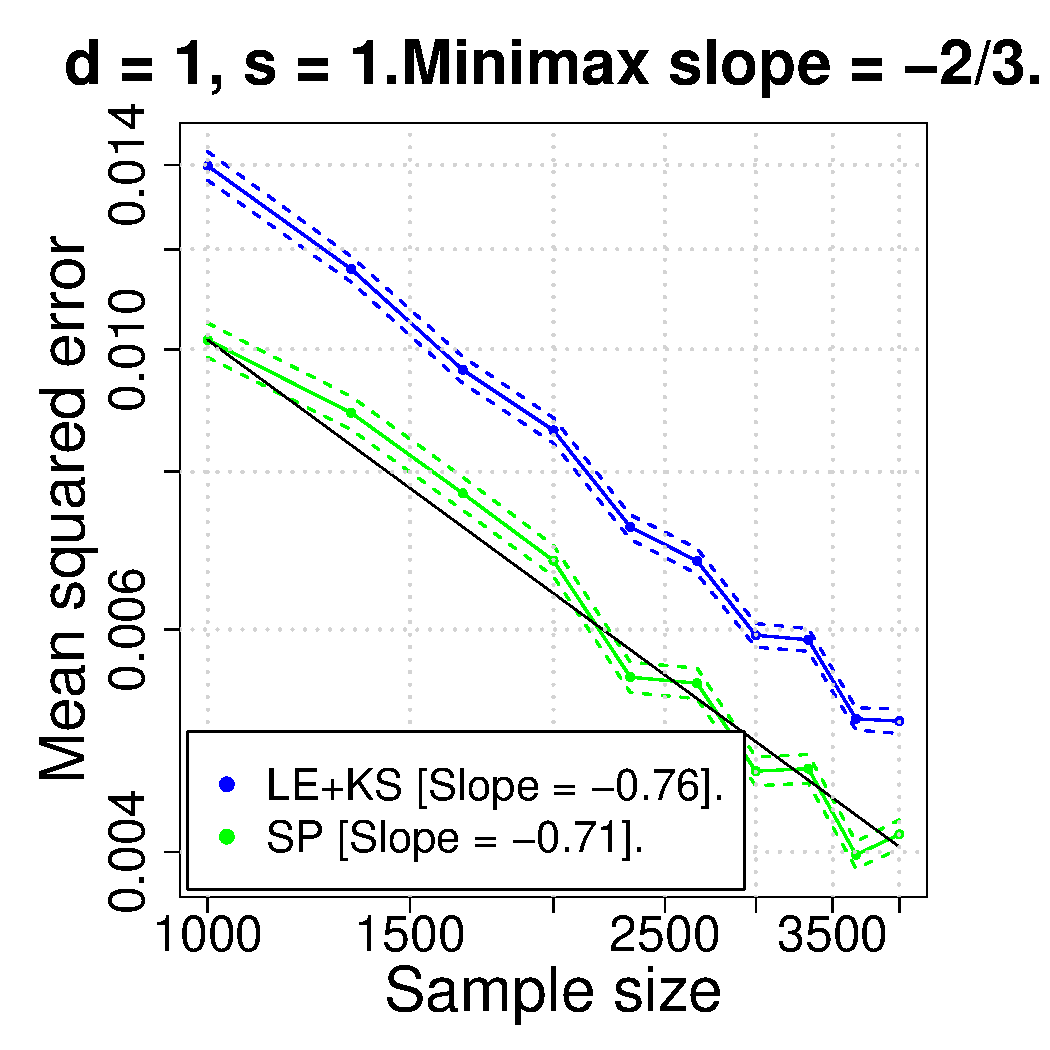
\includegraphics[width=.245\textwidth]{../figures/mse/mse_by_sample_size_1d_1s.pdf}
	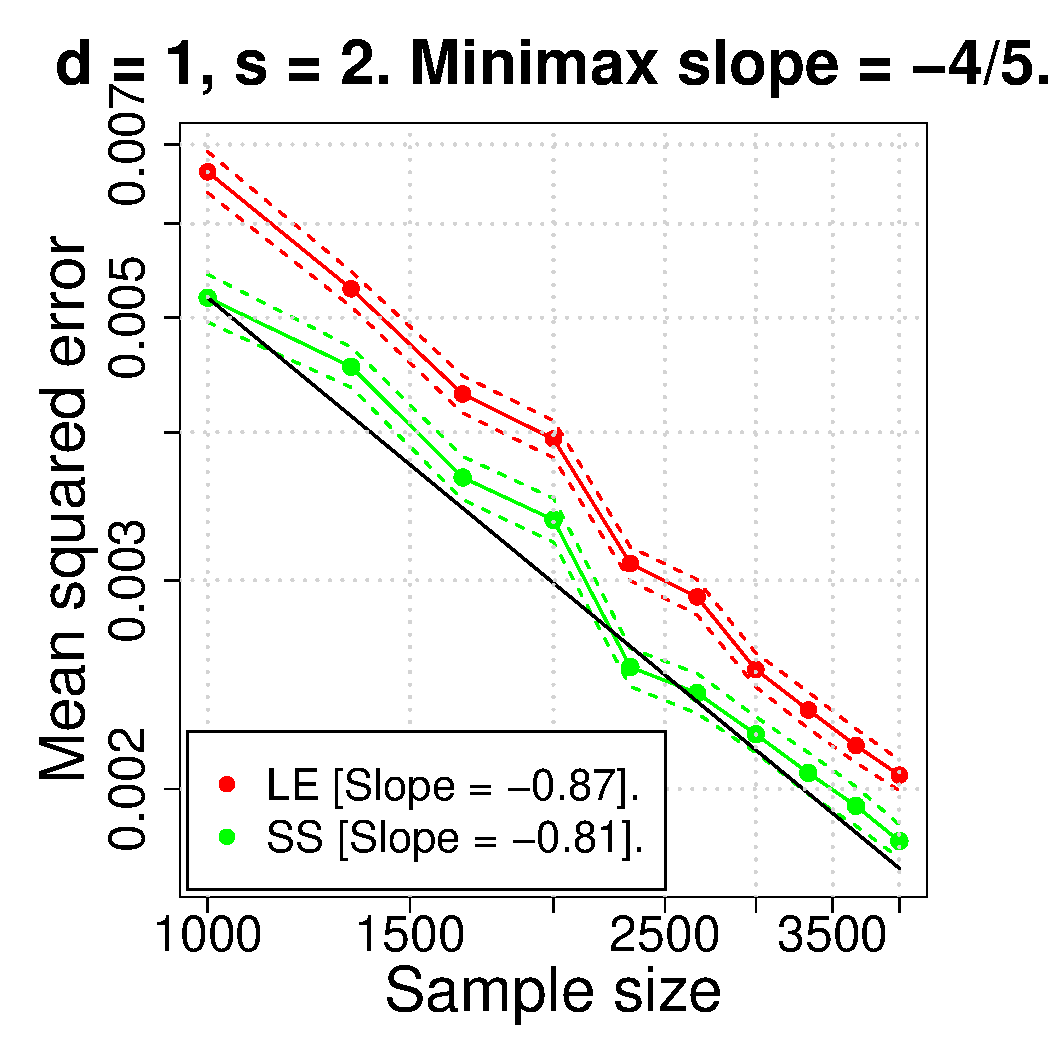
\includegraphics[width=.245\textwidth]{../figures/mse/mse_by_sample_size_1d_2s.pdf}
	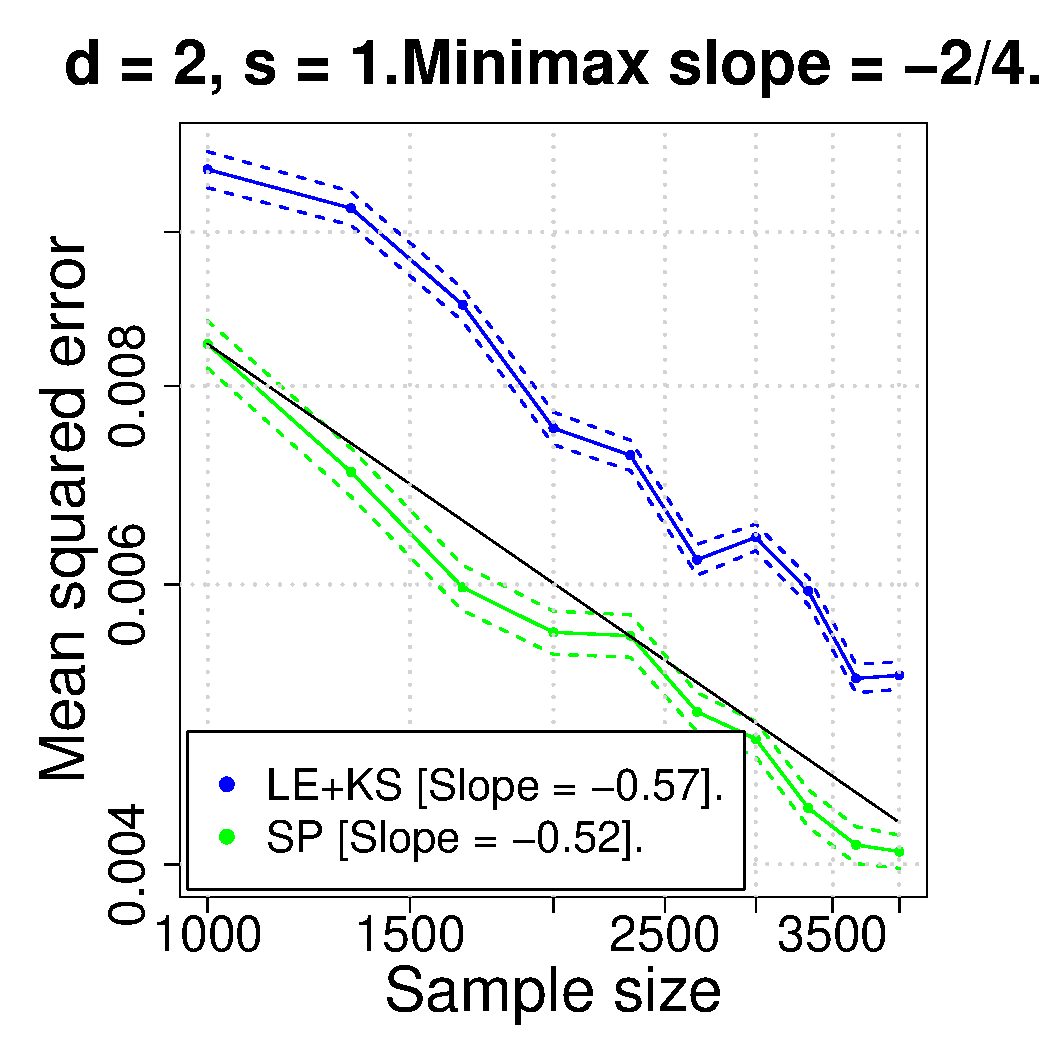
\includegraphics[width=.245\textwidth]{../figures/mse/mse_by_sample_size_2d_1s.pdf}
	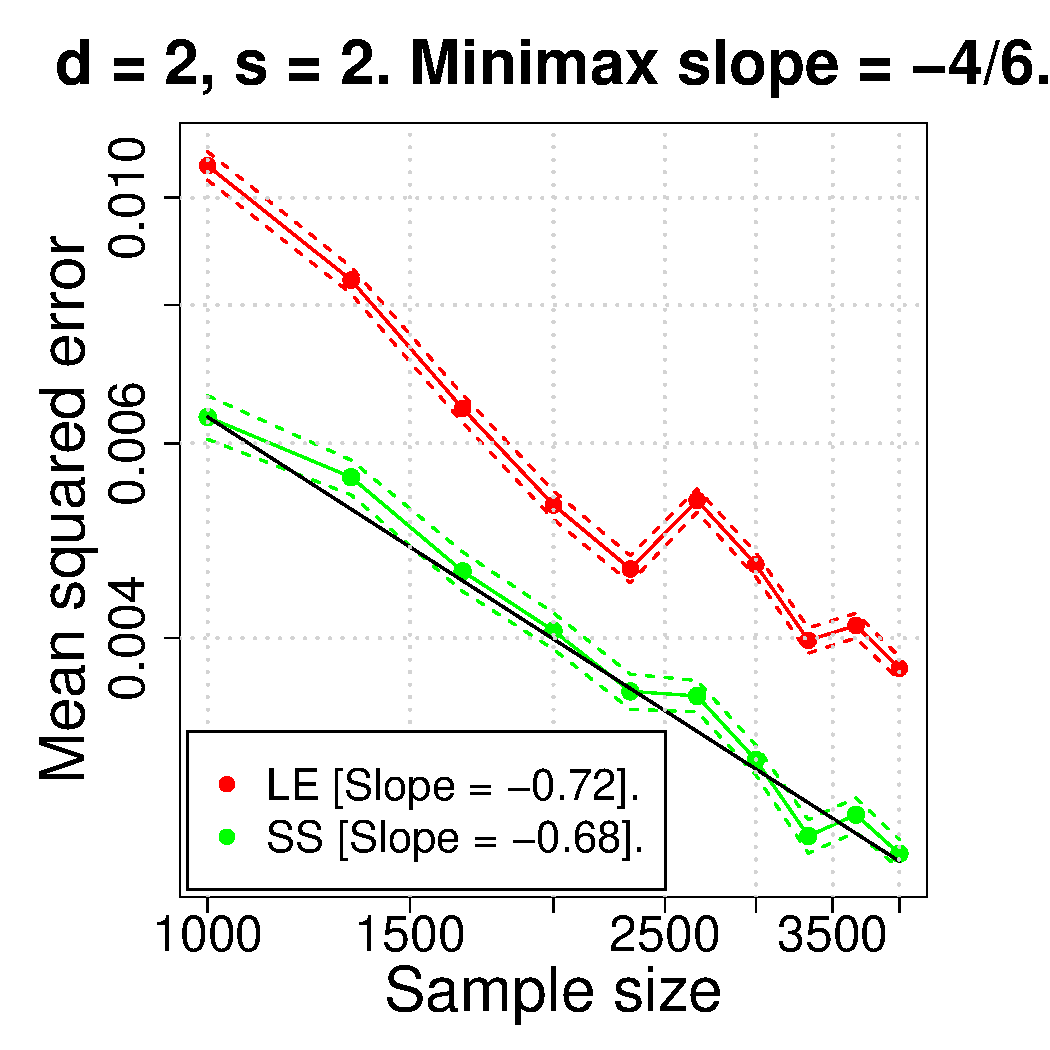
\includegraphics[width=.245\textwidth]{../figures/mse/mse_by_sample_size_2d_2s.pdf}
	\caption{In-sample mean squared error (mse) of PCR-LE (\texttt{LE}) vs. population-level spectral series (\texttt{SS}) estimator, as a function of sample size $n$. Each plot is on the log-log scale, and the results are averaged over 400 repetitions. All estimators are tuned for optimal average mse, separately at each value of $n$. The black line shows the minimax rate (in slope only; the intercept is chosen to match the observed error).}
	\label{fig:fig1}
\end{figure*}

\paragraph{Estimation.}
In our first experiment, we compare the mean-squared error of the PCR-LE estimator $\wh{f}$  to that of its population-level counterpart $\wt{f}$. We vary the sample size from $n = 1000$ to $n = 4000$; sample $n$ design points $\{X_1,\ldots,X_n\}$ from the uniform distribution on the cube $[-1,1]^d$; and sample responses $Y_i$ according to~\eqref{eqn:model} with regression function $f_0 = M/\rho_K^{s/2} \cdot \psi_K$ for $K \asymp n^{d/(2s + d)}$ (the pre-factor $M/\rho_K^{s/2}$ is chosen so that $|f_0|_{H^s(\mc{X})}^2 = M^2$). In Figure~\ref{fig:fig1} we show the in-sample mean-squared error of the two estimators as a function of $n$, for different dimensions $d$ and order of smoothness $s$. We see that both estimators have mean-squared error converging to zero at roughly the minimax rate. While the unsurprisingly population-level spectral series estimator has the smaller error, generally speaking the error of PCR-LE approaches that of the population-level spectral series method as $n$ gets larger. 

\paragraph{Testing.} 
In our second experiment, we compare the PCR-LE test $\varphi$ against the  population-level spectral series test $\wt{\varphi}$. The setup is generally the same as that of our first experiment, but to get an empirical estimate of the critical radius the details are necessarily somewhat more complicated. First we take $\mc{F} = \{M/\rho_k^{s/2} \psi_k\}_{k = 1}^{n}$ to be a discrete subset of $H^1(\mc{X};M)$. Then, for each $f_0 \in \mc{F}$, we run a given test $\phi$ (either the PCR-LE test $\phi = \varphi$, or the population-level spectral series test $\phi = \wt{\varphi}$) and record whether it was a false negative or true positive. We repeat this process over $100$ replications, giving a Monte Carlo estimate of the type II error $E_{f_0}[1 - \phi]$ for each $f_0 \in \mc{F}$. Finally, we take the smallest value of $\|f_0\|_P^2$ such $E_{f_0}[1 - \phi] \leq b$ as our estimate of the critical radius of $\phi$. 

In Figure~\ref{fig:fig2}, we see that the estimated critical radii of both the PCR-LE and population-level spectral series tests are quite close to each other, and converge at roughly the minimax rate.
\begin{figure*}[b]
	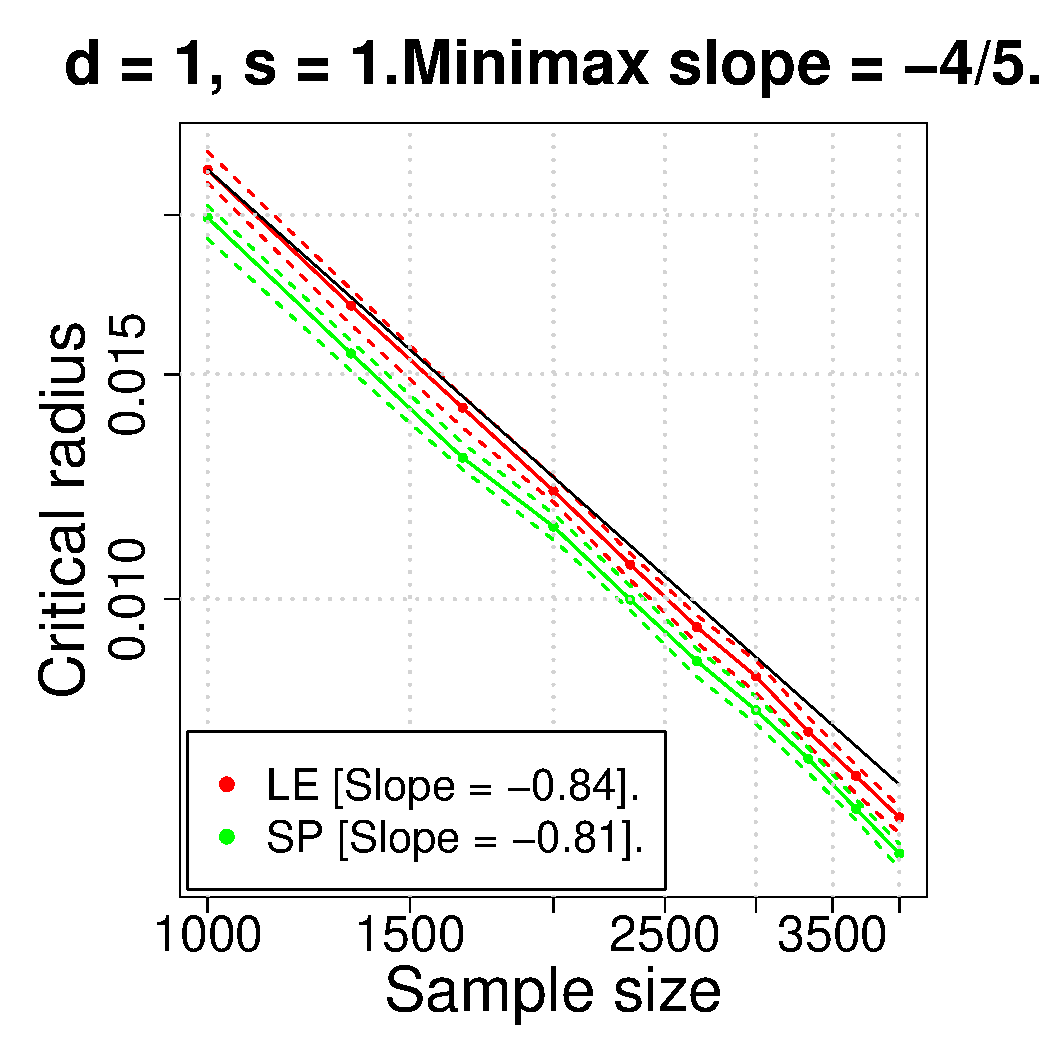
\includegraphics[width=.245\textwidth]{../figures/testing/eigenfunction/critical_radius_by_sample_size_1d_1s.pdf}
	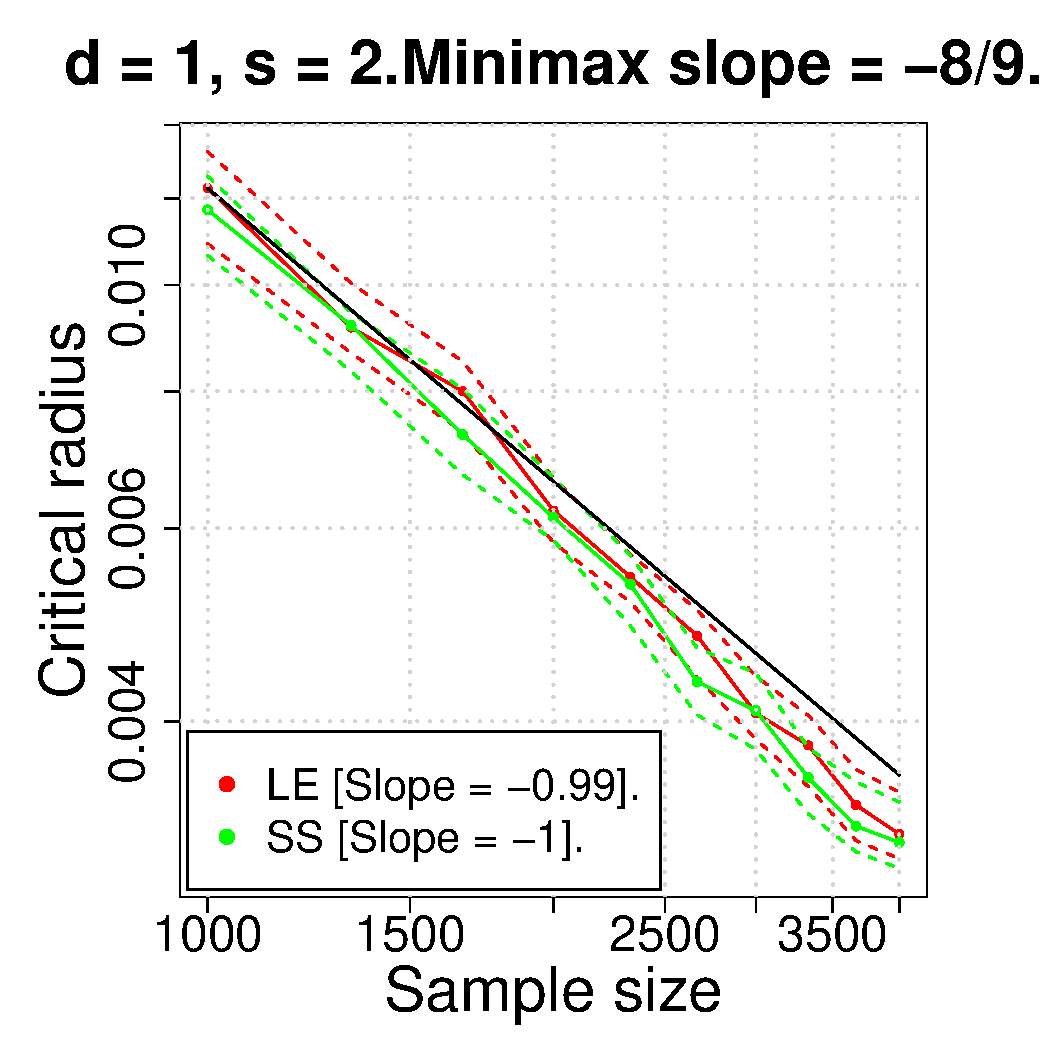
\includegraphics[width=.245\textwidth]{../figures/testing/eigenfunction/critical_radius_by_sample_size_1d_2s.pdf}
	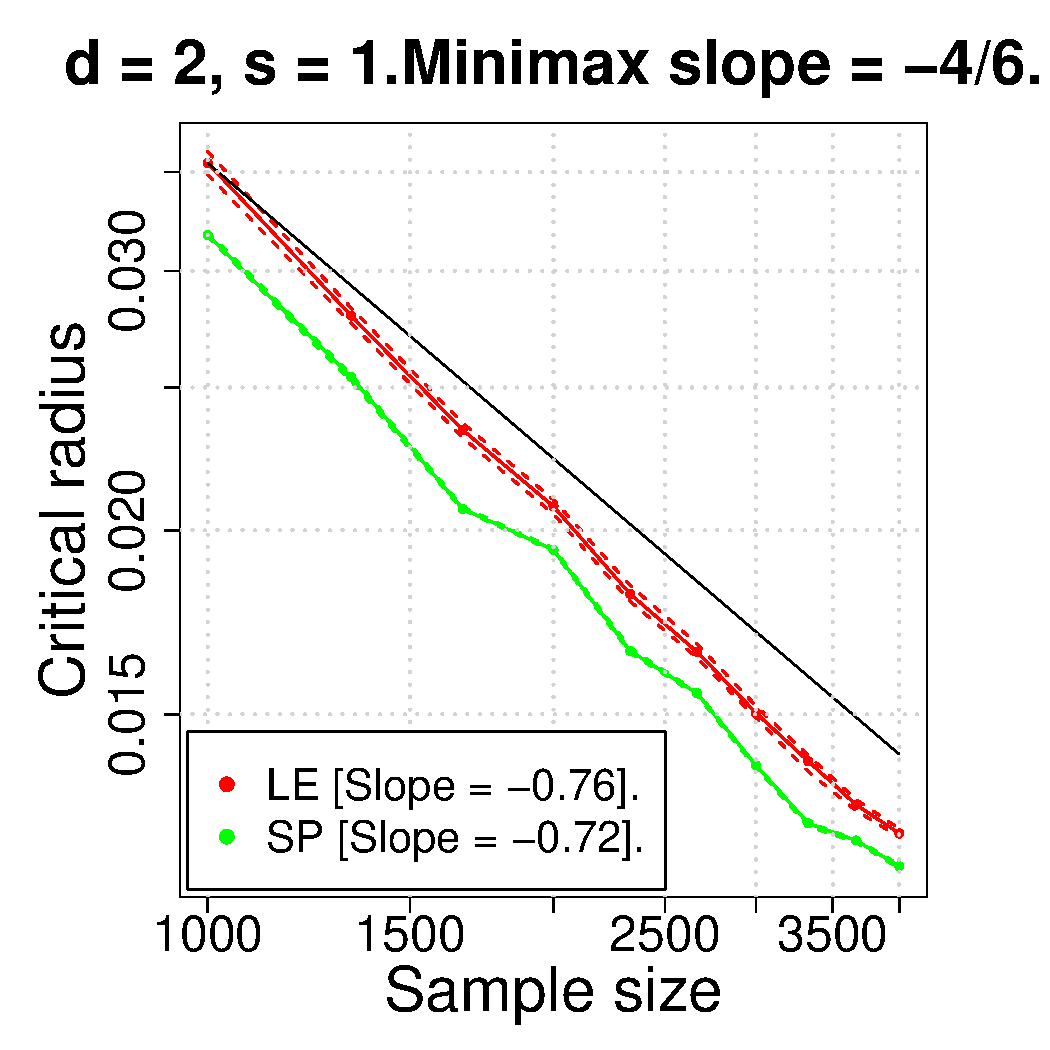
\includegraphics[width=.245\textwidth]{../figures/testing/eigenfunction/critical_radius_by_sample_size_2d_1s.pdf}
	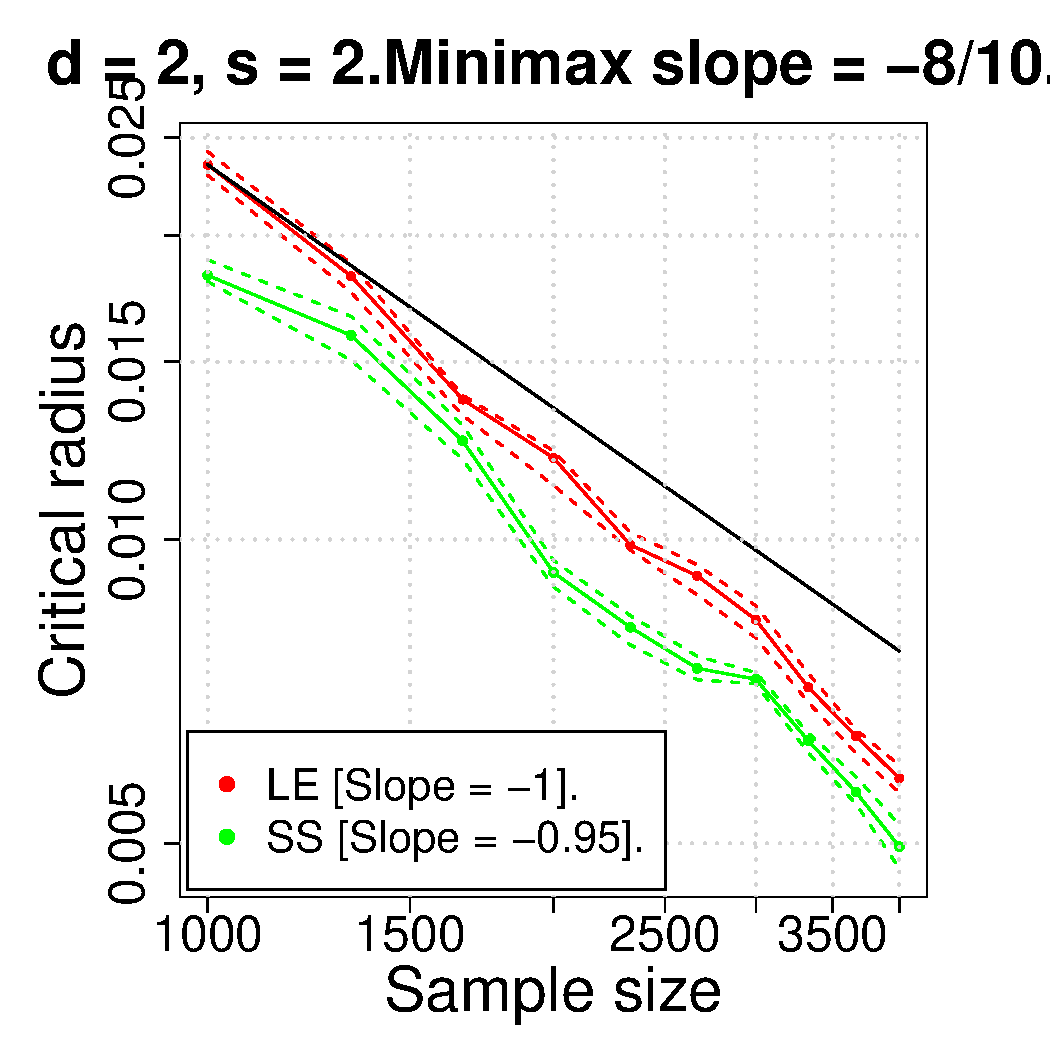
\includegraphics[width=.245\textwidth]{../figures/testing/eigenfunction/critical_radius_by_sample_size_2d_2s.pdf}
	\caption{Worst-case testing risk for PCR-LE (\texttt{LE}) and spectral series (\texttt{SP}) tests, as a function of sample size $n$. Plots are on the same scale as Figure~\ref{fig:fig1}, and black line shows the minimax rate. All tests are set to have $.05$ Type I error, and are calibrated by simulation under the null.}
	\label{fig:fig2}
\end{figure*}

\paragraph{Tuning parameters.}
Our first two experiments demonstrate that PCR-LE methods have comparable statistical performance to population-level spectral series methods. PCR-LE depends on two tuning parameters, and in our final experiment we investigate the importance of both, focusing now on estimation. In Figure~\ref{fig:fig3}, we see how the mean-squared error of PCR-LE changes as each tuning parameter is varied. As suggested by our theory, properly choosing the number of eigenvectors $K$ is crucial: the mean-squared error curves, as a function of $K$, always have a sharply defined minimum. On the other hand, as a function of the graph radius parameter $\varepsilon$ the mean-squared error curve is much closer to flat. This squares completely with our theory, which requires that the number of eigenvectors $K$ be much more carefully tuned that the graph radius $\varepsilon$.

\begin{figure*}[tb]
	\includegraphics[width=.245\textwidth]{../figures/tuning/eigenfunction/mse_by_number_of_eigenvectors_1d_1s.pdf}
	\includegraphics[width=.245\textwidth]{../figures/tuning/eigenfunction/mse_by_radius_1d_1s.pdf} 
	\includegraphics[width=.245\textwidth]{../figures/tuning/eigenfunction/mse_by_number_of_eigenvectors_2d_1s.pdf}
	\includegraphics[width=.245\textwidth]{../figures/tuning/eigenfunction/mse_by_radius_2d_1s.pdf} 
	\includegraphics[width=.245\textwidth]{../figures/tuning/sobolev/mse_by_number_of_eigenvectors_1d_1s.pdf}
	\includegraphics[width=.245\textwidth]{../figures/tuning/sobolev/mse_by_radius_1d_1s.pdf}
	\includegraphics[width=.245\textwidth]{../figures/tuning/sobolev/mse_by_number_of_eigenvectors_2d_1s.pdf}
	\includegraphics[width=.245\textwidth]{../figures/tuning/sobolev/mse_by_radius_2d_1s.pdf}  
	\caption{Mean squared error of PCR-LE (\textcolor{red}{red}), and population-level spectral series (\textcolor{green}{green}) estimators as a function of tuning parameters. Top row: the same regression function $f_0$ as used in Figure~\ref{fig:fig1}. Bottom row: the regression function $f_0 \propto \sum_{k} 1/\rho_k^{1/2} \psi_k$. For all experiments, the sample size $n = 1000$, and the results are averaged over $200$ repetitions. In each panel, all tuning parameters except the one being varied are set to their optimal values.}
	\label{fig:fig3}
\end{figure*}

\section{Discussion}
\label{sec:discussion}

In this work, we have derived upper bounds on the rates of convergence for regression with PCR-LE, which imply that in various settings the PCR-LE estimator and test are minimax rate-optimal over Sobolev classes. Importantly, these upper bounds hold under nonparametric conditions on the design density $p$, and allow for $p$ to be unknown and, potentially, supported on a low-dimensional manifold. Our results help explain the practical success of methods which leverage graph Laplacian eigenvectors for regression. They also distinguish such methods from more traditional spectral series procedures, which rely on a density-dependent basis and thus require the density be known a priori.

Of course, there do exist other methods for nonparametric regression which achieve optimal rates of convergence under similar (or indeed weaker) conditions on $p$. These include other graph-based approaches---Laplacian smoothing---methods besides spectral series methods---e.g. kernel smoothing, local polynomial regression, thin-plate splines---and continuum spectral projection methods which use the eigenfunctions of an operator defined independently of $p$. To be clear, we do not advocate PCR-LE over these alternatives. Rather, we view our results as theoretically justifying a place for regression using Laplacian Eigenmaps in the nonparametric regression toolbox. 

That being said, PCR-LE does have certain advantages over each of the aforementioned approaches. We now conclude by outlining some of these advantages (limiting our discussion to estimation):
\begin{itemize}
	\item \emph{Optimality over high-dimensional Sobolev spaces}. As mentioned in the introduction, Laplacian smoothing (defined via~\eqref{eqn:laplacian_smoothing}) provably achieves minimax optimal rates over $H^1(\mc{X})$ only when $d \in \{1,2,3,4\}$ \citep{sadhanala16, green2021}. In contrast, PCR-LE is optimal over $H^1(\mc{X})$ for all dimensions $d$, and also over the higher-order Sobolev spaces $H^s(\mc{X})$. 
	\item \emph{Manifold adaptivity}. When the design distribution is non-uniform, an oft-recommended alternative to population-level spectral series regression is to run OLS using eigenfunctions of a density-independent differential operator. As a concrete example, let $\Delta$ be the unweighted Laplacian operator on $\Rd$, $\Delta = \sum_{i = 1}^{d} \partial^2f/\partial x_i^2$. Denoting the eigenfunctions of $\Delta$ (under Neumann boundary conditions) by $\phi_1,\phi_2,\ldots$, and letting $\Phi \in \mathbb{R}^{n \times K}$ be the matrix with entries $\Phi_{ik} = \phi_k(X_i)$ and columns $\Phi_1,\ldots,\Phi_K$,  one could compute an estimator by solving the following OLS problem:
	\begin{equation*}
	\minimize_{f \in \mathrm{span}\{\Phi_{1},\ldots,\Phi_{K}\}} \|{\bf Y} - f\|_n^2.
	\end{equation*}
	Unlike with spectral series regression, this approach can produce reasonable estimates even when the sampled eigenfunctions $(\phi_k(X_1),\ldots,\phi_k(X_n)) \in \Reals^n$ are not approximately orthogonal. Indeed, under the conditions of Model~\ref{def:model_flat_euclidean}, such a method will in fact be minimax rate-optimal, though the upper bounds may come with undesirably large constants if $p$ is very non-uniform. However under Model~\ref{def:model_manifold}, this method cannot achieve the faster minimax rates of convergence---which depend only on the intrinsic dimension $m$---and may even be inconsistent. This is because the eigenfunctions $\phi_k$ have no intrinsic relationship to the Sobolev space $H^s(\mc{X})$ except when $\mc{X}$ is a full-dimension set in $\Rd$. In contrast, PCR-LE uses features which are empirical approximations to eigenfunctions $\psi_k$ of the density-weighted Laplace-Beltrami operator $\Delta_P$. The eigenfunctions of $\Delta_P$ are thus adapted to the manifold $\mc{X}$, and PCR-LE is consistent and in certain cases optimal, as we have shown. 
	\item \emph{Density adaptivity}. In Appendix~\ref{subsec:eigenmaps_beats_kernel_smoothing}, we give a simple example of a sequence of densities and regression functions $\{(p^{(n)}, f_0^{(n)}: n \in \mathbb{N}\}$ such that the expected in-sample mean squared error of PCR-LE is smaller than that of either kernel smoothing or least squares using eigenfunctions of $\Delta$. This is possible because PCR-LE induces a completely different bias than these latter two methods. In particular, when $f_0$ and $p$ satisfy the so-called \emph{cluster assumption}---meaning $f_0$ is piecewise constant in high-density regions (clusters) of $p$---then the bias of PCR-LE can be much smaller (for equivalent levels of variance) than that of kernel smoothing or least-squares with eigenfunctions of $\Delta$. 
	
	We emphasize that this does not contradict the well-known optimality properties of, for example, kernel smoothing over H\"{o}lder balls. Rather, in the standard nonparametric regression setup---which we adopt in the main part of this paper, and in which $P$ is assumed to be equivalent to Lebesgue measure---the biases of PCR-LE and kernel smoothing happen to be equivalent. But when $P$ is sufficiently non-uniform, this is no longer the case.
\end{itemize}
Grounding each of these three points on a firmer and more complete theoretical basis would be, in our view, a valuable direction for future work.